\chapter{Formati di trasmissione numerica}

\begin{figure}[h]
    \centering
    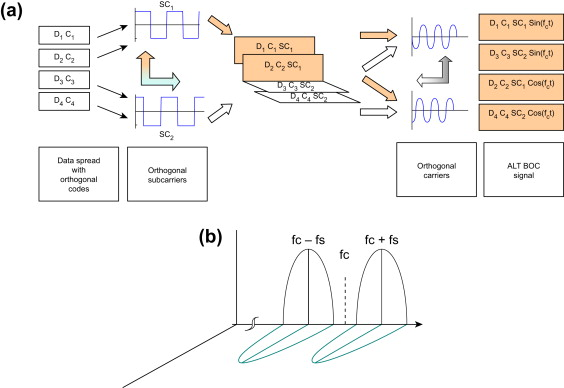
\includegraphics[scale = 1]{orthogonal carrier.jpg}
\end{figure}

\newpage 

\section{Procedura di ortogonalizzazione di Gram-Schmdit}
\footnote{Slide del prof | Formati di trasmissione numerica | pag 1 \\  
Appunti di Damiano | pag 1 \\
Slide | Formati di trasmissione numerica | pag  1\\
Appunti | 2025-03-25 | pag 9
}

\begin{tcolorbox}
    Andando indietro al primo semestre del primo anno di ingegneria elettronica, 
    precisamente al corso di Algebra lineare, abbiamo già visto la procedura di ortogonalizzazione di Gram-Schmidt per costruirci una base vettoriale, cioè lo span dei vettori. \newline 

    Un piccolo ripasso al volo: \\
    \url{https://www.khanacademy.org/math/linear-algebra/alternate-bases/orthonormal-basis/v/linear-algebra-the-gram-schmidt-process} \newline 

    Ma come ci siamo finiti a parlare di segnali come vettori che costituiscono una base ortogonale? \newline 

    All'inizio sembra strano questo concetto, cioè associare segnali che variano nel tempo a vettori, ma poi vedrete che, come la trasformata di Fourier studiata nel corso di Teoria dei Segnali, 
    ci renderà la vita, e specialmente i conti ed i calcoli, più semplice. 
\end{tcolorbox}

Nei vari esempi di rappresentazione di segnali che si è dovuto menzionare, in questo ed altri corsi, 
si è spesso sottolineata, implicitamente o esplicitamente, l'importanza di poter disporre di una base ortogonale. \newline 

\begin{tcolorbox}
    Ripasso da Algebra lineare sotto tre punti di vista: 

    \begin{itemize}
        \item \url{https://youtu.be/k7RM-ot2NWY?si=Iv-U2I81ohPvKAaX} \\ Linear combinations, span, and basis vectors | Chapter 2, Essence of linear algebra by 3Blue1Brown \\ Per capire il concetto, grazie alle animazioni, di cosa si intende per una base vettoriale, i.e. Span 
        \item \url{https://www.andreaminini.org/matematica/spazio-vettoriale/come-trasformare-una-base-in-ortogonale} \\ Come trasformare una base in ortogonale by Andrea Minini  
        \item \url{https://youtu.be/y6Z2EXB2kWQ?si=O4qAQL9ZaQV7eSSp} \\ Base ortogonale , base ortonormale , vettori ortogonali. Ortonormalizzazione di Gram - Schmidt by Salvo Romeo (cioè quella persona che mi salvò e mi fece capire quanto è "facile" Algebra Lineare)
    \end{itemize} 

    Alla fine stiamo parlando dello stesso argomento sotto tre punti di vista differenti.
\end{tcolorbox}

L'esempio più noto, in questo senso, si rinviene nel classico sviluppo in serie di Fourier, 
in cui le funzioni espansione, esponenziali complesse e cosinusoidali, sono appunto ortogonali. \newline 

\begin{tcolorbox}
    Da \url{https://github.com/ciccio25/appunti-teoria-dei-segnali/blob/main/Appunti%20Teoria%20dei%20segnali.pdf} \\
    Capitolo 2.1 - Sviluppo in serie di Fourier - pag 10 - 11 \newline 

    Se il segnale s(t) è periodico con periodo T e pulsazione fondamentale $\omega_0$, possiamo definire una rappresentazione 
nota come Sviluppo in serie di Fourier. \newline 

Il dominio non sarà il tempo, bensì la frequenza (cioè l'inverso del tempo). \newline 

s(t) può essere visto come, grazie alla formula di sintesi dello sviluppo in serie di Fourier: \newline

{
    \Large 
    \begin{equation}
        s(t) 
        = 
        \sum_{k = - \infty}^{\infty} 
        C_k \frac{1}{\sqrt{T}} e^{\jmath \kappa \omega_0 t}
    \end{equation}
}

in cui: \newline

{
    \Large 
    \begin{equation}
        \omega_0 = \frac{2 \pi}{T}
    \end{equation}
}

e $C_k$ viene calcolato dall'analisi dello sviluppo in serie di Fourier: \newline

{
    \Large 
    \begin{equation}
        C_k 
        =
        \frac{1}{\sqrt{T}} \int_{-\frac{T}{2}}^{\frac{T}{2}} 
        s(t) e^{- \jmath \kappa \omega_0 t} dt
    \end{equation}
}

Ricordando, dalla matematica: 

{
    \Large 
    \begin{equation}
        \jmath ^{2} = -1 
    \end{equation}
}


 $e^{\jmath \kappa \omega_0 t}$ rappresenta una sinusoide e ponendo: 

{
    \Large 
    \begin{equation}
        \omega_k = k \omega_0
    \end{equation}
}

possiamo dire che qualsiasi segnale s(t) può essere visto come una 
successione di sinusoidi di diversa pulsazione. \newline 

\end{tcolorbox}

La procedura di ortogonalizzazione di Gram-Schmidt può essere utilizzata per generare un insieme di segnali ortonormali, a partire da un set iniziale di segnali generici. \newline 

\newpage 

\subsection{Due segnali ortogonali e ortonormali}
\footnote{Slide del prof | Formati di trasmissione numerica | pag 1 \\  
Appunti di Damiano | pag 1 \\
Slide | Formati di trasmissione numerica | pag  1\\
Appunti | 2025-03-25 | pag 9
}

Per chiarezza, ricordando che due segnali $s_1 (t)$ e $s_2 (t)$ sono ortogonali se verificano la seguenti proprietà: 

{
    \Large 
    \begin{equation}
        \int s_1 (t) \cdot s_2^{*} (t) dt = 0
    \end{equation}
}

dove: 

\begin{itemize}
    \item per $s_2^{*} (t)$ si intende il complesso coniugato del segnale $s_2 (t)$ 
    \item l'integrale è esteso al dominio comune di definizione tra $s_1 (t)$ e $s_2 (t)$
    \item nel caso più generale, si può assumere un intervallo di integrazione infinito, cioè con $t \in (-\infty, + \infty)$
\end{itemize}

\begin{tcolorbox}
    Dal punto di vista dell'algebra lineare, per vettore complesso coniugato si intende lo stesso vettore con lo stesso modulo, ma fase opposta. \newline
    
    \url{https://www.andreaminini.org/matematica/numeri-complessi/numero-complesso-coniugato} \newline 

    Invece dal punto di vista di calcolo pratico, verificare l'ortogonalità tra $s_1 (t)$ e $s_2 (t)$ significa che  
    dobbiamo considerare $s_2 ^{*} (t)$ con segno opposto di $s_2 (t)$, poi moltiplicare $s_2 ^{*} (t)$ per $s_1 (t)$ e calcolarci l'area (i.e. l'integrale). \newline 
    
    (Un matematico è morto appena ho scritto che calcolare l'integrale significa calcolare l'area sotto ad una funzione. 1 minuto di silenzio. Riposi in pace) \newline 

    Nelle dispense, l'integrale di ortogonalizzazione è scritto con $s_2 (t)$ senza l'asterisco, cioè non si specifica che si intende il suo coniugato: è stato scritto senza per semplicità di notazione, 
    ma ricordatevelo di metterlo. 
\end{tcolorbox}

I segnali $s_1 (t)$ e $s_2 (t)$ non solo possono essere ortogonali, ma possono essere ortonormali se ciascuno di essi è caratterizzato da un'energia $E_i$: 

{
    \Large 
    \begin{equation}
        E_i = \int s_i ^{2} (t) dt \text{ per } i = 1, 2
    \end{equation}
}

che vale 1. \newline 

\newpage 

\subsection{Segnali ortogonali e ortonormali}
\footnote{Slide del prof | Formati di trasmissione numerica | pag 1 - 3\\  
Appunti di Damiano | pag 1 - 3\\
Slide | Formati di trasmissione numerica | pag  1 - 3\\
Appunti | 2025-03-25 | pag 9 
}

Sia dunque dato un insieme M forme d'onda $s_m (t)$ con $1 \le m \le M$. \newline 

Ipotizzando che queste forme d'onda siano utilizzate per la trasmissione dell'informazione in un sistema di comunicazione, 
vogliamo costruire un insieme di $N \le M$ forme d'onda ortonormali, 
che costituiranno la base per lo spazio di dimensione N, 
in cui potranno essere rappresentati, insieme ad altri, gli M segnali di partenza. \newline 

In accordo con la procedura di ortogonalizzazione di Gram-Schmidt, 
si assume la prima forma d'onda $s_1 (t)$ e si costruisce il primo elemento della base ortonormale come $\Psi_1 (t)$: 

{
    \Large 
    \begin{equation}
        \Psi_1 (t) = \frac{s_1 (t)}{\sqrt{E_1}}
    \end{equation}
}

L'energia di $\Psi_1 (t)$ è ovviamente unitaria. \newline 

\begin{tcolorbox}
    La dimostrazione che l'energia di $\Psi_1 (t)$ è unitaria, è la seguente. \newline 

    Considerando $E_{\Psi_1 (t)}$ l'energia di $\Psi_1 (t)$, possiamo calcolarla come: 

    {
        \Large 
        \begin{equation}
            \begin{split}
                E_{\Psi_1 (t)}
                &= 
                \int \left[ \Psi_1 (t) \right]^{2} dt
                \\
                &=
                \int \left( \frac{s_1 (t)}{\sqrt{E_1}}\right)^{2} dt
                \\
                &= 
                \int \frac{s_1 (t) ^{2}}{E_1} dt
                \\
                &=
                \frac{1}{E_1} \cdot \int s_1 (t) ^{2} dt 
                \\
                &= 
                \frac{1}{E_1} \cdot E_1 
                \\
                &= 
                \frac{1}{1}
                \\
                &= 
                1
            \end{split}
        \end{equation}
    }

    (Un altro matematico è morto quando ha visto $\frac{1}{1}$ ma è solo per evidenziare che i due $E_1$ si semplificano)
\end{tcolorbox}

Per valutare il secondo elemento della base, si calcola, innanzitutto, la seguente proprietà: 

{
    \Large 
    \begin{equation}
        c_{21} 
        = 
        \int_{- \infty}^{+ \infty} 
        s_2 (t) \cdot \Psi_1 (t) ^{*} dt
    \end{equation}
}

\begin{tcolorbox}
    Ipotizziamo per adesso, nella formula di $c_{21}$ che l'integrale si estenda per [$-\infty$, $+\infty$] 
\end{tcolorbox}

$c_{21}$ può essere interpretato come la proiezione del segnale $s_2 (t)$ sul primo elemento della base, cioè $\Psi_1 (t)$. \newline 

In pratica, $c_{21}$ è quella parte di $s_2 (t)$ che può essere rappresentata in termini della sola $\Psi_1 (t)$. \newline 

Non a caso: 

{
    \Large 
    \begin{equation}
        \begin{split}
            c_{21} &= 0
            \\
            &\updownarrow
            \\
            s_2 (t) &\perp \Psi_1 (t)
            \\
            \int_{-\infty}^{+\infty}
            s_2 \cdot \Psi_1 (t) ^{*} dt 
            &= 
            0
        \end{split}
    \end{equation}
}

\begin{tcolorbox}
E' ovvio, perchè $\Psi_1 (t)$ si può esprimere come $\frac{s_1 (t)}{\sqrt{E_1}}$ e considerando solo $\frac{1}{\sqrt{E_1}}$ un coefficiente moltiplicativo, 
si ritorna alla formula data nella sezione precedente per due segnale $s_1 (t)$ e $s_2 (t)$ ortogonali.     
\end{tcolorbox}

cioè per esteso, $c_{21}$ è nullo quando $s_2 (t)$ è ortogonale a $\Psi_1 (t)$, 
il che comporta che $\Psi_1 (t)$ non ha alcuna utilità dal punto di vista della rappresentazione di $s_2 (t)$. \newline 

Da quanto procede, risulta chiaro il significato dell'operazione successiva, 
che consiste nel sottrarre a $s_2 (t)$ il prodotto tra $c_{21}$ e $\Psi_1 (t)$. \newline 

Formalmente $d_2 (t)$ vale:

{
    \Large
    \begin{equation}
        d_2 (t)
        = 
        s_2 (t) 
        - 
        c_{21} \cdot \Psi_1 (t)
    \end{equation}
}

\begin{tcolorbox}
    Se $c_{21} \cdot \Psi_1 (t) = 0$, allora $d_2 (t) = s_2 (t)$, cioè abbiamo una nuova funzione di base 
\end{tcolorbox}

$d_2 (t)$ è certamente ortogonale a $\Psi_1 (t)$, avendo infatti: 

{
    \Large 
    \begin{equation}
        \begin{split}
            \int_{-\infty}^{+ \infty}
            d_2 (t)
            \cdot 
            \Psi_1 (t)
            dt 
            &= 
            \int_{-\infty}^{+ \infty}
            \left[
                s_2 (t) - c_{21} \cdot \Psi_1 (t)
            \right]
            \cdot 
            \Psi_1 (t)
            dt 
            \\
            &=
             \int_{-\infty}^{+ \infty}
            s_2 (t) 
            \cdot 
            \Psi_1 (t)
            dt 
            -
            c_{21}
            \cdot
            \int_{-\infty}^{+ \infty}
            \Psi_1 ^{2} (t)
            dt 
            \\
            &=
            c_{21} - c_{21} \cdot 1 
            \\
            &= 
            c_{21} - c_{21}
            \\
            &= 
            0
        \end{split}
    \end{equation}
}

\begin{tcolorbox}
    In questa equazione non sono stati messi i complessi coniugati, ma fai finta che ci siano.
\end{tcolorbox}

$d_2 (t)$ non ha energia unitaria. \newline 


Per costruire, a partire da esso, una funzione ortonormale, 
ottenendo in tal modo il secondo elemento della base, 
valutiamo la sua energia, definita convenzionalmente come $E_2$: 

{
    \Large 
    \begin{equation}
        E_2 = \int_{- \infty}^{+ \infty} \left[ d_2 (t) \right]^{2} dt
    \end{equation}
}

Si potrà allora scrivere $\Psi_2 (t)$: 

{
    \Large 
    \begin{equation}
        \Psi_2 (t) = \frac{d_2 (t)}{\sqrt{E_2}}
    \end{equation}
}

e questa è una ortogonale a $\Psi_1 (t)$ ed ha energia unitaria. \newline 

Se: 

{
    \Large 
    \begin{equation}
        d_2 (t) \neq 0
    \end{equation}
}

$\Psi_2 (t)$ può essere assunta come secondo elemento della base. \newline 

La procedura descritta può essere generalizzata, ponendo: 

{
    \Large 
    \begin{equation}
        \Psi_k (t) = \frac{d_k (t)}{\sqrt{E_k}}
    \end{equation}
} 

In questa espressione si ha: 

{
    \Large 
    \begin{equation}
        d_k (t)
        = 
        s_k (t) 
        - 
        \sum_{i = 1}^{k-1}
        c_{ki} \cdot \Psi_i (t)
    \end{equation}
}

e: 

{
    \Large 
    \begin{equation}
        E_k = \int_{- \infty}^{+ \infty} \left[ d_k (t) \right]^{2}
    \end{equation}
}

con: 

{
    \Large 
    \begin{equation}
        c_{ki}
        = 
        \int_{-\infty}^{+ \infty}
        s_k \cdot \Psi_{i} dt
    \end{equation}
}


Confrontando la formula di $d_k (t)$ e di $c_{ki}$ afferma qualitativamente che il contributo del segnale $s_k (t)$ alla costruzione della base ortonormale 
è dovuto alla parte del segnale che non è già rappresentabile utilizzando una combinazione lineare delle funzioni di base già determinate. \newline 

La procedura appena descritta va ripetuta per tutti i segnali $s_m (t)$, in cui $1 \le m \le M$. \newline 

La cardinalità N della base (ovvero il numero degli elementi che la costituiscono) sarà uguale a M (la cardinalità dell'insieme di partenza) 
se gli M segnali $s_m (t)$ sono tra loro linearmente indipendenti: 
vale a dire che nessuno di essi può essere ottenuto per combinazione lineare degli altri. \newline 

Ciò è sicuramente vero quando gli M segnali sono tra loro ortogonali. \newline 

Se tutti i segnali sono ortogonali, si ha sempre N = M. \newline 

\newpage 

\subsection{Segnali come combinazione lineare della base N-dimensione}
\footnote{Slide del prof | Formati di trasmissione numerica | pag 4 - 6\\  
Appunti di Damiano | pag 4 - 6\\
Slide | Formati di trasmissione numerica | pag  4 - 6\\
Appunti | 2025-03-25 | pag 9 - 10
}

Una volta costituito il set di forme d'onda ortogonali, 
cioè l'insieme $\{ \Psi_k (t) \} $, 
gli M segnali $s_m (t)$ possono essere espressi come combinazione lineare delle funzioni della base, 
in accordo con la seguente formula generale: 

{
    \Large 
    \begin{equation}
        s_m (t) 
        = 
        \sum_{k = 1}^{N}
        s_{mk} \cdot \Psi_{k} (t)
    \end{equation}
}

\begin{tcolorbox}
    Come nella rappresentazione in Serie di Fourier in cui si rappresentano i segnali con i loro coefficienti, 
    anche qui si rappresentano i segnali con le loro basi $\Psi_k (t)$ finite (con k che parte da 1 e va fino a N funzioni di base)
\end{tcolorbox}

L'orto-normalità della base rende semplice il calcolo dei coefficienti dell'espansione, $s_{mk}$, 
per i quali si avrà infatti: 

{
    \Large
    \begin{equation}
        s_{mk}
        = 
        \int_{-\infty}^{+ \infty}
        s_{m} (t) \cdot \Psi_{k} (t) dt
    \end{equation}
}

La medesima proprietà è poi alla base del calcolo dell'energia, 
in accordo con la formula seguente: 

{
    \Large 
    \begin{equation}
        \begin{split}
            E_{m}
            &= 
            \int_{- \infty}^{+ \infty}
            \left[ s_{m} (t) \right]^{2} dt 
            \\
            &= 
            \sum_{k = 1}^{N} (s_{mk})^{2}
        \end{split}
    \end{equation}
}

In accordo con la teoria generale della rappresentazione di un segnale secondo una base assegnata, 
le proprietà del segnale (ad esempio la sua energia), possono essere ricavate indifferentemente, 
dalla conoscenza diretta del segnale o dei parametri della sua rappresentazione. \newline 

\begin{tcolorbox}
    Come avevamo ribadito nel corso di Teoria dei Segnali \newline 

    \url{https://github.com/ciccio25/appunti-teoria-dei-segnali/blob/main/Appunti%20Teoria%20dei%20segnali.pdf} \\
    Capitolo 2.1 - Sviluppo in serie di Fourier \newline 

    Diverse volte è utile osservare lo stesso segnale in altre rappresentazioni equivalenti. \newline 

    Per rappresentazione di un segnale si intende una qualsiasi modalità idonea alla sua individuazione 
    biunivoca. \newline 

    La rappresentazione può comportare un cambiamento del dominio di definizione. \newline  

    Quindi, grazie ad una rappresentazione, si può passare da un dominio all'altro dello stesso segnale. \newline 

\end{tcolorbox}

Dal punto di vista geometrico, la formula di $s_{m} (t)$ è evidente: 
le funzioni $\Psi_{k} (t)$ con k = 1, 2, $\dots$, N, possono essere riguardate come altrettanti versori che definiscono uno spazio N-dimensionale, 
sopra il quale la generica forma d'onda $s_{m} (t)$ è rappresentata tramite le sue componenti. \newline 

\begin{tcolorbox}
    Ripasso al volo su cosa si intende per base vettoriale dal corso di Algebra Lineare e le sue proprietà: \\
    \url{https://www.andreaminini.org/matematica/spazio-vettoriale/base-algebra-lineare} 
\end{tcolorbox}

Raccolte in un vettore, possiamo scrivere le componenti della generica forma d'onda $s_{m} (t)$ come: 

{
    \Large 
    \begin{equation}
        \overrightarrow{s_{m}} 
        = 
        (s_{m1}, s_{m2}, \dots, s_{mN})
    \end{equation}
}

\begin{tcolorbox}
    Piccola precisazione di notazione. \newline 

    In tutti i corsi fatti in cui si ha a che fare con i vettori, 
    ogni corso, quindi ogni professore, ha la propria simbologia per rappresentarli. \newline 

    Il prof, nelle sue dispense, utilizza il grassetto per differenziare il vettore dalle sue componenti. \newline 

    Io invece, personalmente, sono abituato a indicare il vettore con la freccia sopra, 
    perchè, quando scrivo a mano le notazioni matematiche (ad esempio durante uno scritto o durante l'orale) 
    riesco a distinguere al volo cosa è un vettore e cosa no. \newline 
    
    Fate come volete, l'importante è utilizzare una notazione che sia costante. 
\end{tcolorbox}

Nello spazio N-dimensionale identificato dalla base, 
il segnale $s_{m} (t)$ è rappresentato da un punto, 
le cui coordinate sono le componenti $s_{mN}$ data dalla formula di $\overrightarrow{s_m}$. \newline 

L'utilizzo delle componenti consente anche di esprimere il prodotto intero tra due segnali come: 

{
    \Large 
    \begin{equation}
        \begin{split}
            \int_{- \infty}^{+ \infty}
            s_{m} (t) \cdot s_{n} (t) dt
            &= 
            \overrightarrow{s_m} \cdot \overrightarrow{s_n}
            \\
            &= 
            \sum_{k = 1}^{N}
            s_{mk} \cdot s_{nk}
        \end{split}
    \end{equation}
}

dove: 

\begin{itemize}
    \item per $\overrightarrow{s_m} \cdot \overrightarrow{s_n}$ si intende il prodotto scalare tra i vettori $\overrightarrow{s_m}$ e $\overrightarrow{s_n}$
    \item per $\sum_{k = 1}^{N} s_{mk} \cdot s_{nk}$ si intende la somma tra i singoli componenti dei due vettori $\overrightarrow{s_m}$ e $\overrightarrow{s_n}$
\end{itemize}

\begin{tcolorbox}
    Piccolo ripasso da Algebra lineare per cosa si intende prodotto scalare. \newline 

    \url{https://www.youtube.com/watch?v=LyGKycYT2v0&t=30s} \\
    Dot products and duality | Chapter 9, Essence of linear algebra by 3Blue1Brown \newline 

    \url{https://youtu.be/UqpY07EiwCU?si=Fj_7MjStUPMHjvSx}\\ 
    Dot Product (1 of 2: Geometric interpretation) by Eddie Woo
\end{tcolorbox}

In definitiva, l'espansione in funzioni ortonormali è uno strumento assolutamente utile sia alla rappresentazione della classe di segnali considerata, 
sia ai fini della valutazioni delle loro proprietà, 
sia ai fini della loro elaborazione e combinazione. \newline 

In effetti, l'espansione in funzioni ortogonali è uno dei presupposti per la migliore descrizione dei sistemi di trasmissione numerici, 
ove i segnali che portano l'informazione sono rappresentati da forme d'onda di durata limitata T. \newline 

Infine, è opportuno osservare che, per un dato insieme di segnali $s_{m} (t)$, 
l'insieme delle forme d'onda che definisce la base ortonormale non è necessariamente unico. \newline 

L'importante è che il cambiamento di base non fa cambiare la dimensione dello spazio e l'energia di ciascun segnale o il prodotto intero tra una qualunque coppia di vettori. \newline 

In definitiva, l'algoritmo di ortogonalizzazione di Gram-Schmidt garantisce la generazione di una base ortonormale per la rappresentazione di un dato insieme di segnali. \newline

Ma non per questo dobbiamo sempre applicare questo algoritmo per individuare una base ortonormale. \newline 

\begin{tcolorbox}
    Detta in altre parole, se è la tua ultima spiaggia, utilizza l'algoritmo Gram-Schmdit, sennò, utilizza altri algoritmi.
\end{tcolorbox}

\newpage 

\section{Esempi di segnali in spazi N-dimensionali}
\footnote{Slide del prof | Formati di trasmissione numerica | pag 8 \\  
Appunti di Damiano | pag 8 \\
Slide | Formati di trasmissione numerica | pag  8\\
Appunti | 2025-03-28 | pag 2
}

Assegnato un insieme di M segnali $s_m (t)$, in cui $1 \le m \le M$, 
è sempre possibile rappresentare ciascuno di essi in uno spazio di dimensione N individuato (e quindi descritto) da N forme d'onda ortonormali $\Psi_i (t)$, 
in cui $1 \le i \le N$. \newline 

In un sistema di comunicazione numerico, ciascun segnale $s_m (t)$, denominato simbolo, 
può essere associato alla trasmissione di k bit, dove k vale: 

{
    \Large 
    \begin{equation}
        k = \log_{2} (M)
    \end{equation}
}

Visto che la sorgente emetterà una sequenza binaria, quindi di 0 e 1, 
ciascun bit avendo durata $T_B$, ciascun simbolo avrà durata pari a T, dove T vale: 

{
    \Large 
    \begin{equation}
        T = k \cdot T_B
    \end{equation}
}

Le caratteristiche della trasmissione, dal punto di vista della qualità (cioè in presenza di rumore o altri disturbi sovrapposti), 
dell'occupazione spettrale e altre caratteristiche della trasmissione, 
dipendono, per un dato valore di M, dalla dimensione dello spazio e, 
per un dato N, dalla distribuzione dei segnali (loro punti rappresentativi) all'interno dello spazio. \newline 

\newpage

\section{Segnali in spazi di dimensione N = 1}
\footnote{Slide del prof | Formati di trasmissione numerica | pag 8 - 10\\  
Appunti di Damiano | pag 8 - 10\\
Slide | Formati di trasmissione numerica | pag  8 - 10\\
Appunti | 2025-03-28 | pag 2 - 6 \\
Appunti | 2025-07-21 Ricevimento | pag 4
}

In questo caso, lo spazio è unidimensionale, ed è generato da una sola funzione espansione $\Psi_1 (t)$. \newline 

I segnali $s_m (t)$ sono proporzionali a tale funzione. \newline 

Una possibile distribuzione dei punti (che può essere anche chiamata come costellazione) 
sull'asse che identifica lo spazio è la seguente: 

\begin{figure}[h]
    \centering
    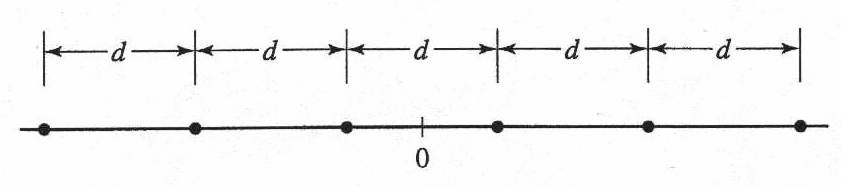
\includegraphics[scale = 1]{Spazio dimensionale N = 1.png}
\end{figure}

Come si vede dalla figura, i punti sono distribuiti simmetricamente rispetto all'origine, 
a distanza d l'uno dall'altro. \newline 

Come funzione di base $\Psi_1 (t)$ si può assumere: 

{
    \Large 
    \begin{equation}
        \Psi_1 (t) = \frac{1}{\sqrt{E_g}} \cdot g_{T} (t) \text{ per } 0 \le t \le T
    \end{equation}
}

dove: 

\begin{itemize}
    \item $g_T (t)$ è una funzione generica 
    \item $E_g$ è l'energia di $g_T (t)$
\end{itemize}

La forma di $g_T (t)$ può essere scelta con l'intento di ottenere, ad esempio, un'occupazione spettrale consona alla disponibilità di banda. \newline 

Ad esempio $g_T (t)$ può avere questo andamento: 

\begin{figure}[h]
    \centering
    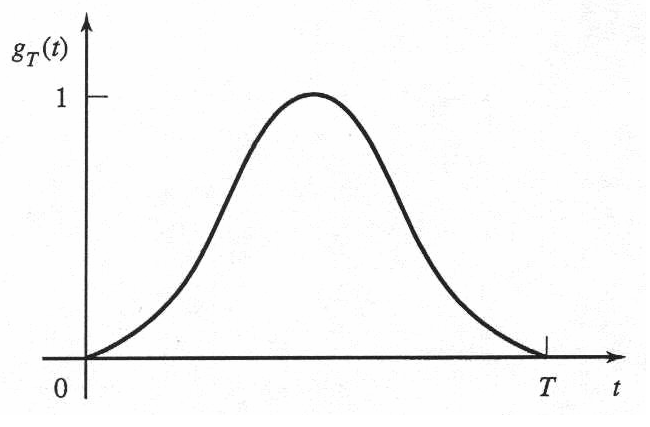
\includegraphics[scale = 0.7]{Andamento di un segnale come base.png}
\end{figure}

\newpage 

Ma, frequentemente, si assume per $g_T (t)$ un impulso rettangolare

\begin{figure}[h]
    \centering
    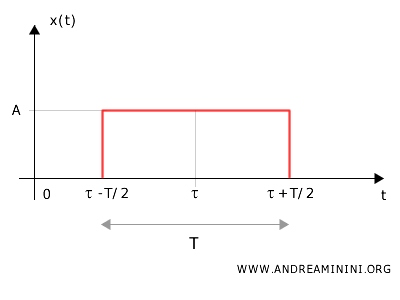
\includegraphics[scale = 0.7]{il-segnale-rettangolare-nelle-te.jpg}
\end{figure} 

con andamento: 

{
    \Large 
    \begin{equation}
        g_T (t)
        = 
        \begin{cases}
            \sqrt{\frac{E_g}{T}} \text{ per } 0 \le t \le T 
            \\
            \quad
            \\
            0 \text{ altrove}
        \end{cases}
    \end{equation}
}

\begin{tcolorbox}
    A rigore, quindi in un contesto reale di un sistema di telecomunicazioni, non si utilizzeranno gli impulsi rettangolari, 
    perchè, dalle proprietà tra tempo e frequenza: \newline 

    \url{https://github.com/ciccio25/appunti-teoria-dei-segnali/blob/main/Appunti%20Teoria%20dei%20segnali.pdf} \\
    Capitolo 3.4 - Altre caratteristiche sulla dualità tempo-frequenza - pag 24 \newline 

     \begin{itemize}
        \item Un segnale s(t) che è limitato nel tempo, ha spettro illimitato sull'asse delle pulsazioni 
        \item Un segnale con spettro delle pulsazioni limitato, ha un'evoluzione temporale illimitata in t. \\ 
     \end{itemize}

     $\blacksquare$ \newline 

Quindi a rigore useremo $g_T (t)$ gaussiana vista precedentemente, 
ma siccome "telecomunicazioni" è "un corso di base", consideriamo gli impulsi rettangolari, 
anche perchè sono molto più semplici da trattare matematicamente con i calcoli.

\end{tcolorbox}

Da quanto precede, si deduca che il generico segnale $s_m (t)$ può essere scritto come: 

{
    \Large 
    \begin{equation}
        s_{m} (t) = s_m \cdot \Psi_1(t)
    \end{equation}
}


Sapendo che c'è una funzione di base $\Psi_1 (t)$, 
i segnali $s_m (t)$ differiscono solo per l'ampiezza ed a quanto sono proporzionali da $\Psi_1 (t)$, 
quindi significa anche essere proporzionali a $g_T (t)$. \newline 

Sapendo ciò, possiamo scrivere: 

{
    \Large 
    \begin{equation}
        s_m (t)
        = 
        A_m \cdot g_T (t) \text{ per } m = 1, 2, \dots, M \text{ e } 0 \le t \le T
    \end{equation}

}

Il coefficiente $s_m$ si ottiene facilmente come segue: 

{
    \Large 
    \begin{equation}
        \begin{split}
            s_m 
            &= 
            \int_{0}^{T}
            s_m \cdot \Psi_1 (t) dt
            \\
            &= 
            \int_{0}^{T}
            \left[A_m \cdot g_T (t) \right] 
            \cdot 
            \left[ \frac{g_T (t)}{\sqrt{E_g}}\right]
            dt
            \\
            &=
            \int_{0}^{T}
            A_m \cdot \frac{\left[g_T (t) \right]^{2}}{\sqrt{E_g}} dt
            \\
            &=
            \frac{A_m}{\sqrt{E_g}}
            \cdot 
            \int_{0}^{T}
            \left[g_T (t) \right]^{2}
            dt
            \\
            &=
            \frac{A_m}{\sqrt{E_g}}
            \cdot
            E_g
            \\
            &= 
            A_m \cdot \sqrt{E_g} 
        \end{split}
    \end{equation}
}

\begin{tcolorbox}

    Per coefficiente $s_m$ si intende un coefficiente della base ortogonale e ortonormale per rappresentare i segnali ad N-dimensione

\end{tcolorbox}

In quanto discriminanti dall'ampiezza, 
i segnali $s_m (t)$ hanno diversa energia. \newline 

Risulta infatti che l'energia $E_m$ di un segnale $s_m$ si possa calcolare come: 

{
    \Large 
    \begin{equation}
        \begin{split}
            E_m 
            &= 
            (s_m)^{2}
            \\
            &= 
            \left[ A_m \cdot \sqrt{E_g} \right]^{2}
            \\
            &= 
            A_m ^{2} \cdot E_g 
            \\
            &= 
            E_g \cdot A_m ^{2}   
        \end{split}
    \end{equation}
}

In alcune applicazioni, in particolare per lo studio dei sistemi di telecomunicazione, 
ha interesse considerare l'energia media della costellazione $E_{av}$, definita come: 

{
    \Large 
    \begin{equation}
        \begin{split}
            E_{av}
            &=
            \frac{1}{M} 
            \cdot 
            \sum_{m = 1}^{M} 
            E_m
            \\
            &= 
            \frac{1}{M} 
            \cdot 
            \sum_{m = 1}^{M} 
            E_g \cdot A_m ^{2}
            \\
            &= 
            \frac{E_g}{M}
            \cdot 
            \sum_{m = 1}^{M}
            A_m ^{2}
        \end{split}
    \end{equation}
}


\begin{tcolorbox}
    $E_{av}$, av, dall'inglese, si intende average che significa media
\end{tcolorbox}

\newpage 

Nel caso di punti simmetricamente disposti rispetto all'origine come in figura: 

\begin{figure}[h]
    \centering
    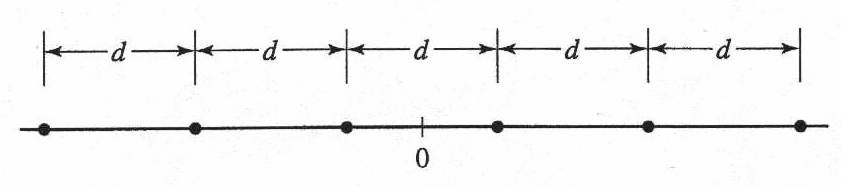
\includegraphics[scale = 0.6]{Spazio dimensionale N = 1.png}
\end{figure}

l'ampiezza del singolo segnale è $A_m$: 

{
    \Large 
    \begin{equation}
        A_m 
        = 
        \left( 2 \cdot m - 1 - M\right)
    \end{equation}
}

e quindi, la potenza media della costellazione $E_{av}$ diventa: 

{
    \Large 
    \begin{equation}
        \begin{split}
            E_{av}
            &= 
            \frac{E_g}{M}
            \cdot
            \sum_{m = 1}^{M}
            A_m ^{2}
            \\
            &= 
            \frac{E_g}{M}
            \cdot
            \sum_{m = 1}^{M}
            \left( 2 \cdot m - 1 - M\right)^{2}
            \\
            &= 
            \dots
            \\
            &= 
            \frac{E_g \cdot \left(M^{2} - 1\right)}{3}
        \end{split}
    \end{equation}
}

Infine, la radice quadrata della distanza Euclidea tra due punti della costellazione vale: 

{
    \Large 
    \begin{equation}
        \begin{split}
            d_{mn}
            &= 
            \sqrt{\abs{s_m - s_n}^{2}}
            \\
            &= 
            \sqrt{E_g \cdot \left(A_m - A_n\right)^{2}}
        \end{split}
    \end{equation}
}

dove: 

\begin{itemize}
    \item $s_m$ e $s_n$ sono due punti nella costellazione 
    \item $A_m$ e $A_n$ sono, rispettivamente, le ampiezze dei punti $s_m$ e $s_n$ 
\end{itemize}

\begin{tcolorbox}
    Ricordiamo che, nella formula di $d_{mn}$, $s_m$ e $s_n$ sono scalari
\end{tcolorbox}

Maggiore sarà la distanza tra i punti della costellazione, 
più semplice sarà per il ricevitore capire la differenza tra i vari simboli 
(ma maggiore distanza significa anche che il trasmettitore dovrà utilizzare più energia per inviare i simboli). \newline 

\newpage 

\subsubsection{Esempi di modulazioni con N = 1}
\footnote{Slide del prof | Formati di trasmissione numerica | pag 10 - 11\\  
Appunti di Damiano | pag 10 - 11\\
Slide | Formati di trasmissione numerica | pag  10 - 11\\
Appunti | 2025-03-28 | pag 6 - 8
}

Queste considerazioni vengono svolte per una trasmissione in banda base. \newline 

Questo tipo di trasmissione prende il nome di PAM (Pulse Amplitude Modulation), 
che è una modulazione in banda base che, come dice il nome, ogni simbolo viene contraddistinto in base alla sua ampiezza. \newline 

Considerando M = 2, 
possiamo considerare una 2-PAM, in cui andamento dei segnali è il seguente: 

\begin{figure}[h]
    \centering
    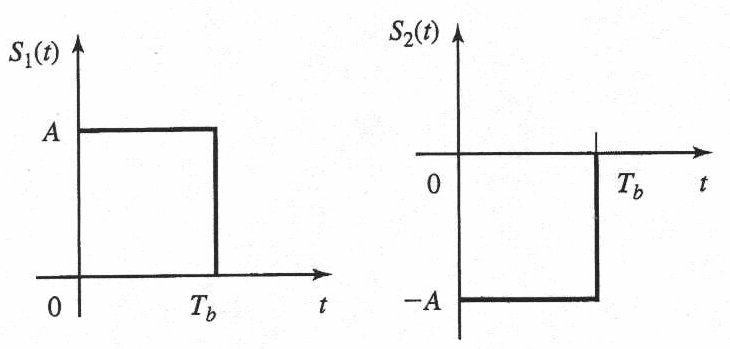
\includegraphics[scale = 0.6]{2 PAM.png}
\end{figure}

Se invece si considera M = 4, 
possiamo considerare una 4-PAM, in cui andamento dei segnali è il seguente: 

\begin{figure}[h]
    \centering
    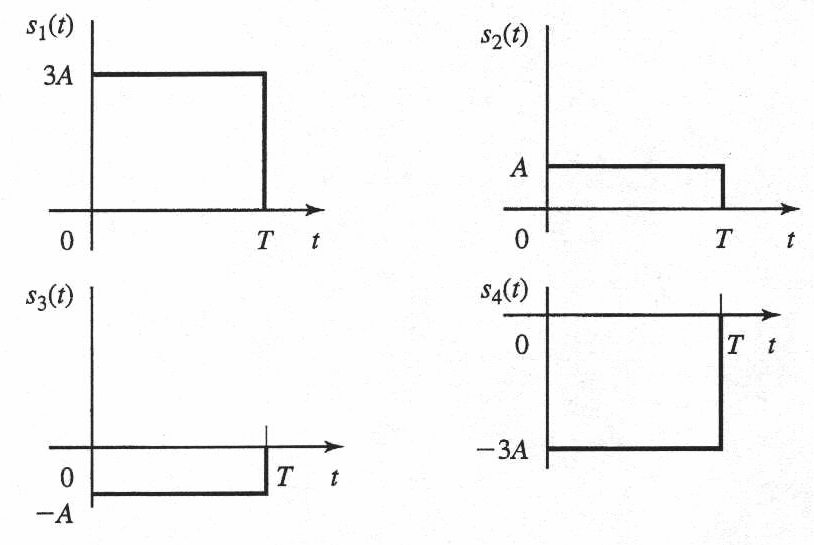
\includegraphics[scale = 0.6]{4 PAM.png}
\end{figure}

Invece, se moduliamo il segnale M-PAM a una sinusoide $\cos(2 \pi f_c t)$, 
otteniamo il segnale $u_m (t)$ traslato in $2 \pi f_c$, 
che si ottiene come: 

{
    \Large 
    \begin{equation}
        u_m (t)
        =
        A_m \cdot g_T (t) \cdot \cos(2 \pi f_c t) \text{ per } m = 1, 2, \dots, M \text{ e } 0 \le t \le T
    \end{equation}
}

Se consideriamo il caso particolare in cui $g_T (t)$ è un impulso rettangolare, cioè: 

{
    \Large 
    \begin{equation}
        g_T (t)
        = 
        \begin{cases}
            \sqrt{\frac{E_g}{T}} \text{ per } 0 \le t \le T 
            \\
            \quad
            \\
            0 \text{ altrove}
        \end{cases}
    \end{equation}
}

$u_m (t)$ sarà un segnale ASK (Amplitude Shift Keying). \newline 

\newpage 

Un generico andamento di un segnale ASK, nel caso di M = 2, è il seguente (con le note): 

\begin{figure}[h]
    \centering
    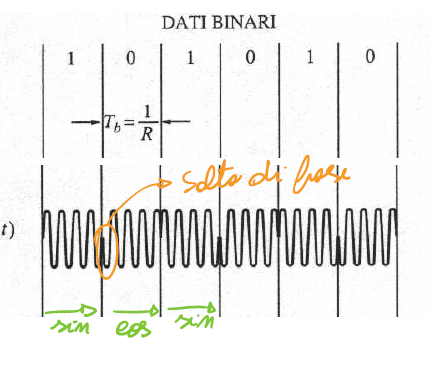
\includegraphics[scale = 1]{2 ASK andamento segnale.PNG}
\end{figure}

In effetti il caso ASK binario merita particolare menzione. \newline 

Esso è caratterizzato da forme d'onda antipodale (il coefficiente di correlazione vale -1) e si tratta di un formato di trasmissione che garantisce prestazioni estremamente elevate. \newline 

Sempre per il caso binario, in luogo di forme d'onda antipodali, 
è possibile assumere forme d'onda ortogonali (coefficiente di correlazione uguale a 0). \newline 

Il risultato si consegue associando alla trasmissione di uno dei due livelli logici la forma d'onda nulla. \newline 

Questo tipo di trasmissione prende il nome di OOK (On-Off Keying). \newline 

Un esempio di un andamento di un segnale in OOK: 

\begin{figure}[h]
    \centering
    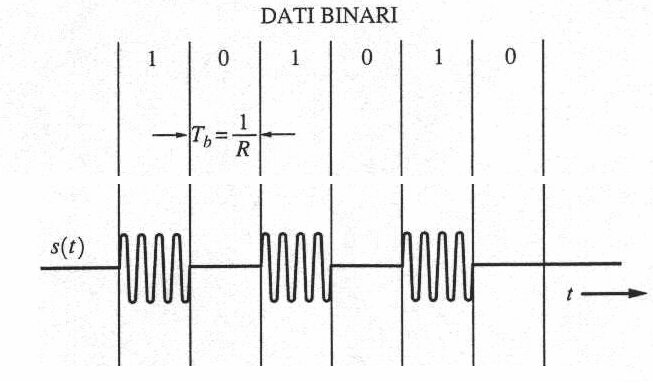
\includegraphics[scale = 0.8]{OOK andamento segnale.png}
\end{figure}

La OOK è un formato meno efficiente della 2-ASK (a parità degli altri parametri), 
ma risulta più semplice da implementare. \newline 

Ad esempio la OOK è implementata nella fibra ottica, dove la presenza di luce si intende 1, 
l'assenza di luce si intende 0. \newline 

In generale, possiamo dire che la OOK e la ASK sono formati monodimensionali perchè hanno una funzione di base. \newline 

\begin{tcolorbox}
    Un altro modo per visualizzare e capire cosa è una funzione di base, 
    pensiamo quali sono le caratteristiche che permettono di contraddistinguere i vari simboli uno dall'altro. \newline 

    Ad esempio, nella OOK, l'unico parametro che permette di distinguere il simbolo da un altro è la presenza o meno della portante $\cos(2 \pi f_c t)$. \newline 

    Nella ASK, l'unico parametro che permette di contraddistinguere il simbolo da un altro è la sua fase. \newline 

    Nella PAM, l'unico parametro che permette di contraddistinguere il simbolo da un altro è la sua ampiezza. \newline 

    Sembra banale, ma adesso che andremo a visualizzare formati di trasmissione in cui N è maggiore di 1, le considerazioni da svolgere saranno diverse e più complesse. \newline 

    L'importante è avere dei concetti di base, e per cosa si intende per base, solide e semplici. 
\end{tcolorbox}

\newpage 

\section{Segnali in spazi di dimensione N = 2}
\footnote{Slide del prof | Formati di trasmissione numerica | pag 11 - 14\\  
Appunti di Damiano | pag 11 - 14\\
Slide | Formati di trasmissione numerica | pag  11 - 14\\
Appunti | 2025-03-28 | pag 8 
}

In questo caso, lo spazio è bidimensionale, ed è generato da due funzioni espansione $\Psi_1 (t)$ e $\Psi_2 (t)$. \newline 

Considerando due coppie di segnali, cioè: 

\begin{itemize}
    \item prima coppia è $s_1 (t)$ e $s_2 (t)$
    \item seconda coppia è $s_1^{'} (t)$ e $s_2^{'} (t)$
\end{itemize} 

e visualizzando il loro andamento nelle seguenti figure: 

\begin{figure}[h]
    \centering
    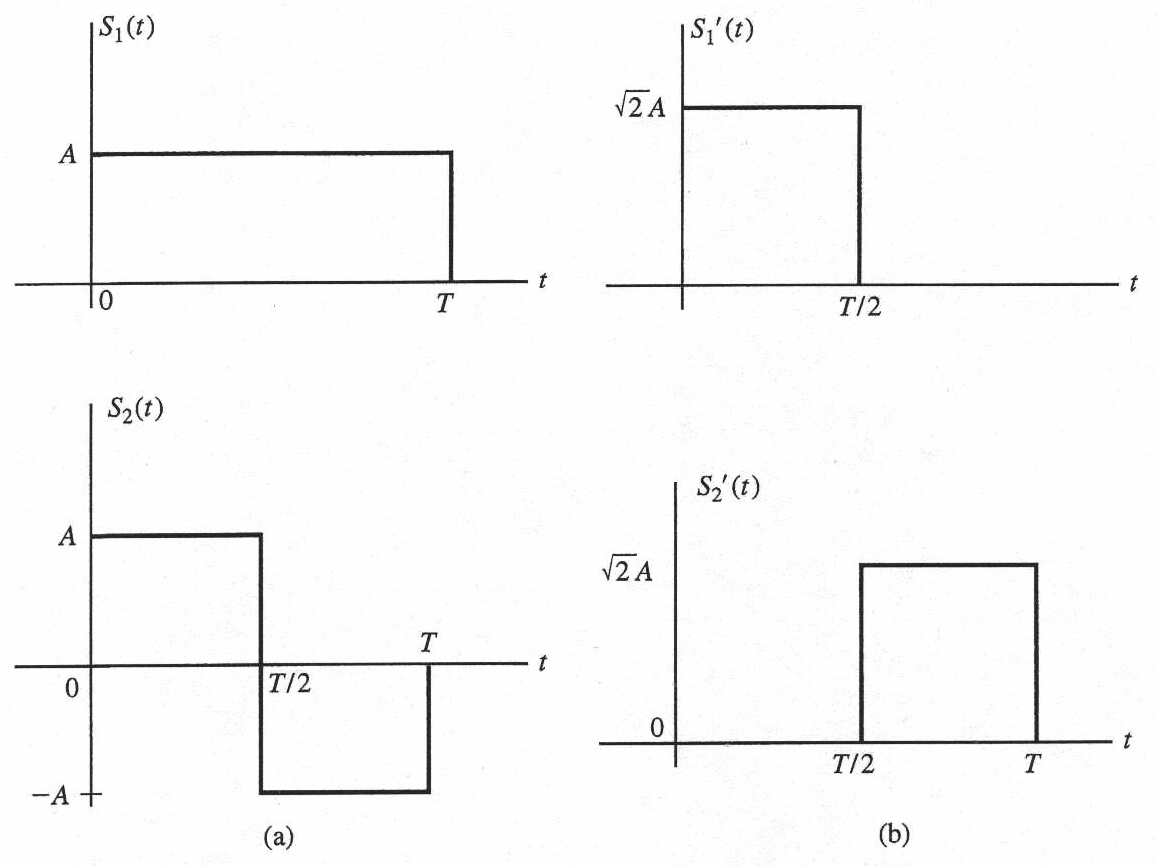
\includegraphics[scale = 0.6]{Segnali N = 2.png}
\end{figure}

possiamo verificare la condizione di ortogonalità: 

{
    \Large 
    \begin{equation}
        \int_{0}^{T}
        s_1 (t) \cdot s_2^{*} (t) 
        dt 
        =
        \int_{0}^{T}
        s_1^{'} (t) \cdot \left[s_2^{'} (t) \right]^{*}  
        dt 
        = 
        0
    \end{equation}
}

Inoltre, l'energia di tutte le forme d'onda elementari considerare è la stessa e vale: 

{
    \Large 
    \begin{equation}
        \begin{split}
            E 
            &= 
            \int_{0}^{T}
            s_1^{2} (t)
            dt
            \\
            &= 
            \int_{0}^{T}
            s_2^{2} (t)
            dt
            \\
            &= 
            \int_{0}^{T}
            \left[ s_1^{'} (t) \right]^{2} 
            dt
            \\
            &= 
            \int_{0}^{T}
            \left[ s_2^{'} (t) \right]^{2}
            dt
            \\
            &=
            A^{2} \cdot T
        \end{split}
    \end{equation}
}

\begin{tcolorbox}
    Ricordati la regola aurea dell'ingegnere: per calcolare l'energia di un segnale, 
    cioè l'integrale in un periodo T, devi prendere l'ampiezza del segnale in quel periodo, elevarlo alla seconda perchè stiamo parlando di potenze, 
    e moltiplicarlo per il periodo T, proprio come se stessi calcolando l'area di un rettangolo 
\end{tcolorbox}

Grazie all'ortogonalità, 
si può presupporre che: 

{
    \Large 
    \begin{equation}
        N = M = 2
    \end{equation}
}

In altre parole, non sarebbe possibile aggiungere un ulteriore segnale ortogonale senza aumentare la dimensione della base. \newline 

Lo spazio bidimensionale in cui rappresentare i segnali analizzati, 
cioè i segnali $s_1 (t)$, $s_2 (t)$, $s_1^{'} (t)$ e $s_2^{'} (t)$, 
può essere generato, ad esempio, dalle seguenti funzioni rettangolari: 

{
    \Large 
    \begin{equation}
        \begin{cases}
            \Psi_1 (t)
            = 
            \begin{cases}
                \sqrt{\frac{2}{T}} \text{ per } 0 \le t \le \frac{T}{2}
                \\
                0 \text{ altrove}
            \end{cases}
            \\
            \quad
            \\
            \Psi_2 (t)
             = 
            \begin{cases}
                \sqrt{\frac{2}{T}} \text{ per } \frac{T}{2} \le t \le T
                \\
                0 \text{ altrove}
            \end{cases}
        \end{cases}
    \end{equation}
}

\begin{tcolorbox}
    Ricordiamo sul perchè il prof ha scritto "ad esempio". \newline 

    La procedura di ortogonalizzazione di Gram-Schmidt ci garantisce che va bene qualsiasi segnale come base dello spazio, 
    basta che poi i segnali che si trovano in quello spazio siano combinazione lineare dei versori della base stessa
\end{tcolorbox}

\newpage 

Dal punto di vista grafico, 
possiamo visualizzare l'andamento nel tempo di $\Psi_1 (t)$ come: 

\begin{figure}[h]
    \centering
    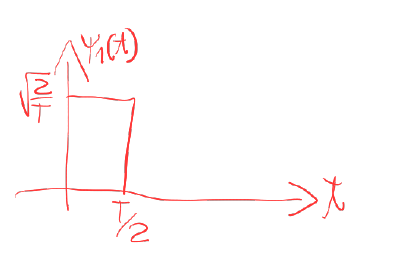
\includegraphics[scale = 1]{Prima funzione di base per N = 2.PNG}
\end{figure}

Invece, l'andamento nel tempo di $\Psi_2 (t)$ come: 

\begin{figure}[h]
    \centering
    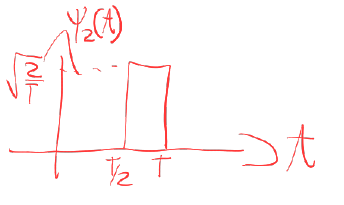
\includegraphics[scale = 1]{Seconda funzione di base per N = 2.PNG}
\end{figure}

Allora, le forme d'onda $s_1 (t)$ e $s_2 (t)$, ad esempio, si esprimono come: 

{
    \Large 
    \begin{equation}
        \begin{cases}
            s_1 (t) = s_{11} \cdot \Psi_1(t) + s_{12} \Psi_2 (t)
            \\
            \quad
            \\
            s_2 (t) = s_{21} \cdot \Psi_1(t) + s_{22} \Psi_2 (t)
        \end{cases}
    \end{equation}
}

ovvero, come si verifica immediatamente, tramite le loro componenti nello spazio bidimensionale: 

{
    \Large 
    \begin{equation}
        \begin{cases}
            \overrightarrow{s_1} = (s_{11}, s_{12} ) = \left(A \cdot \sqrt{\frac{T}{2}}, A \cdot \sqrt{\frac{T}{2}}\right)
            \\
            \quad
            \\
            \overrightarrow{s_2} = (s_{21}, s_{22} ) = \left(A \cdot \sqrt{\frac{T}{2}}, -A \cdot \sqrt{\frac{T}{2}}\right)
        \end{cases}
    \end{equation}
}

Possiamo visualizzare $\overrightarrow{s_1}$ e $\overrightarrow{s_2}$ su un piano bidimensionale in questa maniera: 

\begin{figure}[h]
    \centering
    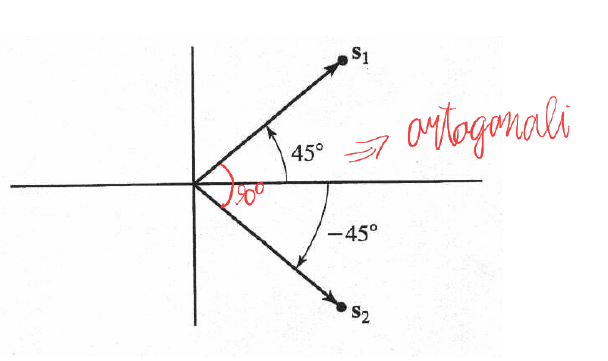
\includegraphics[scale = 1]{Piano bidimensionale dei coefficienti di Fourier in un piano N =2.PNG}
\end{figure}

I due segnali $\overrightarrow{s_1}$ e $\overrightarrow{s_2}$ sono rappresentati da vettori che sono tra loro ortogonali. \newline 

La lunghezza di ogni vettore al quadrato, fornisce l'energia di ciascun segnale. \newline 

Cioè: 

{
    \Large 
    \begin{equation}
        \begin{cases}
        E_1 = \abs{\overrightarrow{s_1}}^{2}
        \\
        \quad
        \\
        E_2 = \abs{\overrightarrow{s_2}}^{2}
        \end{cases}
    \end{equation}
}


dove con $\abs{\overrightarrow{s_1}}$ e $\abs{\overrightarrow{s_2}}$ si intendono i moduli, 
cioè la lunghezza dei vettori $\overrightarrow{s_1}$ e $\overrightarrow{s_2}$. \newline 

La radice quadrata della distanza Euclidea tra i due segnali $d_{12}$, in questo caso, vale: 

{
    \Large 
    \begin{equation}
        \begin{split}
            d_{12}
            &= 
            \sqrt{\abs{\overrightarrow{s_1} - \overrightarrow{s_2}}^{2}}
            \\
            &= 
            \dots
            \\
            &= 
            A \cdot \sqrt{2 \cdot T}
        \end{split}
    \end{equation}
}

Sapendo che l'energia E vale: 

{
    \Large 
    \begin{equation}
        E = A^{2} \cdot T
    \end{equation}
}

possiamo riscrivere la distanza Euclidea $d_{12}$ in funzione dell'energia E anche come: 

{
    \Large
    \begin{equation}
        \begin{split}
            d_{12} 
            &= 
            A \cdot \sqrt{2 \cdot T}
            \\
            &= 
            \sqrt{2 \cdot E}
        \end{split}
    \end{equation}
}

\begin{tcolorbox}
    Comparando la distanza tra i due vettori in N = 1: 

    {
        \Large 
        \begin{equation}
            d_{12} = 2 \cdot \sqrt{E}
        \end{equation}
    }

    nel caso N = 2, 
    la distanza tra i due vettori è diminuita perchè $\sqrt{2 \cdot E}$ è minore rispetto a $\sqrt{E}$. \newline 

    Lo si può anche notare dalle raffigurazioni nello spazio bidimensionale. \newline 

    I due vettori, piuttosto che avere una differenza di $180^{\circ}$, 
    differiscono solo di $90^{\circ}$. \newline 

    Questo "avvicinamento" peggiore la probabilità di errore dei simboli, ma è più facile da implementare rispetto al caso N = 1. \newline 

    Quindi, come ogni argomento di questo corso e di ogni corso di ingegneria, bisogna scegliere sul momento della progettazione quale criterio ci interessa di più ai nostri scopi, 
    cioè, e lo ripeterò allo sfinimento, non puoi avere la moglie ubriaca e la botta piena contemporaneamente. \newline 
    
    La vita reale è fatta di compromessi. \newline 

    La dimostrazione di $d_{12}$ è semplice se parti da $\sqrt{2 \cdot E}$ e fai il processo inverso
\end{tcolorbox}

\newpage 

Utilizzando la stessa base $\Psi_1 (t)$ e $\Psi_2 (t)$: 

{
    \Large 
    \begin{equation}
        \begin{cases}
            \Psi_1 (t)
            = 
            \begin{cases}
                \sqrt{\frac{2}{T}} \text{ per } 0 \le t \le \frac{T}{2}
                \\
                0 \text{ altrove}
            \end{cases}
            \\
            \quad
            \\
            \Psi_2 (t)
             = 
            \begin{cases}
                \sqrt{\frac{2}{T}} \text{ per } \frac{T}{2} \le t \le T
                \\
                0 \text{ altrove}
            \end{cases}
        \end{cases}
    \end{equation}
}

e facendo gli stessi passaggi precedenti, cioè: 

{
    \Large 
    \begin{equation}
        \begin{cases}
            s_1^{'} (t) = s_{11}^{'} \cdot \Psi_1(t) + s_{12}^{'} \Psi_2 (t)
            \\
            \quad
            \\
            s_2^{'} (t) = s_{21}^{'} \cdot \Psi_1(t) + s_{22}^{'} \Psi_2 (t)
        \end{cases}
    \end{equation}
}

possiamo esprimere $s_1^{'} (t)$ e $s_2^{'} (t)$ come: 

{
    \Large 
    \begin{equation}
        \begin{cases}
            \overrightarrow{s_1^{'}} = (s_{11}^{'}, s_{12}^{'} ) = \left(A \cdot \sqrt{T}, 0 \right) = \left( \sqrt{E}, 0\right)
            \\
            \quad
            \\
            \overrightarrow{s_2^{'}} = (s_{21}^{'}, s_{22}^{'} ) = \left(0 , A \cdot \sqrt{T}\right) = \left( 0 , \sqrt{E}\right)
        \end{cases}
    \end{equation}
}

La corrispondente rappresentazione grafica nello spazio bidimensionale di $\overrightarrow{s_1^{'}}$ e $\overrightarrow{s_2^{'}}$ è la seguente: 

\begin{figure}[h]
    \centering
    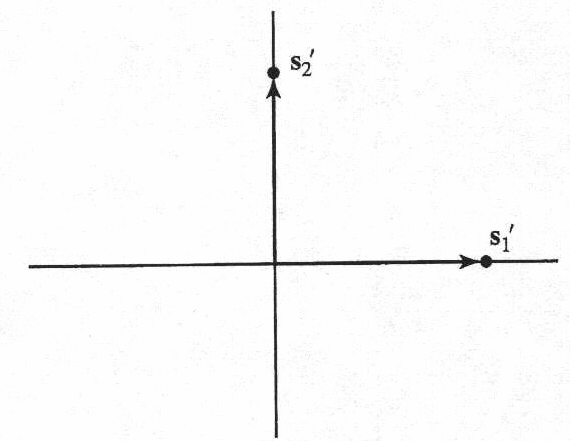
\includegraphics[scale = 1]{Piano bidimensionale dei coefficienti di Fourier in un piano N =2 stessa base.PNG}
\end{figure}

Stante la similitudine tra le due rappresentazione, cioè quella di $\overrightarrow{s_1}$ con $\overrightarrow{s_2}$, 
la distanza Euclidea tra $\overrightarrow{s_1^{'}}$ e $\overrightarrow{s_2^{'}}$ è la stessa di $\overrightarrow{s_1}$ e $\overrightarrow{s_2}$, cioè: 

{
    \Large 
    \begin{equation}
        d_{1^{'}2^{'}} = d_{12}
    \end{equation}
}

e inoltre, la rappresentazione dei due vettori $\overrightarrow{s_1^{'}}$ e $\overrightarrow{s_2^{'}}$ 
è la stessa di $\overrightarrow{s_1}$ e $\overrightarrow{s_2}$ con una semplice rotazione di $45^{\circ}$. \newline 

\newpage 

\subsection{Esempio di modulazione con N = 2: la PPM}
\footnote{Slide del prof | Formati di trasmissione numerica | pag 14 \\  
Appunti di Damiano | pag 14 \\
Slide | Formati di trasmissione numerica | pag  14\\
Appunti | 2025-03-28 | pag 8
}

Un esempio di modulazione con N = 2, è la PPM (Pulse Position Modulation). \newline 

Dato il piano bidimensionale, i segnali differiscono per la posizione dell'impulso. \newline 

L'ortogonalità può essere conseguita facendo in maniere tale che i due impulsi non si sovrappongono. \newline 

Un esempio di due segnali che non si sovrappongono, li avevamo visti precedentemente con $s_1^{'} (t)$ e $s_2^{'} (t)$, 
in cui andamento nel tempo è il seguente: 

\begin{figure}[h]
    \centering
    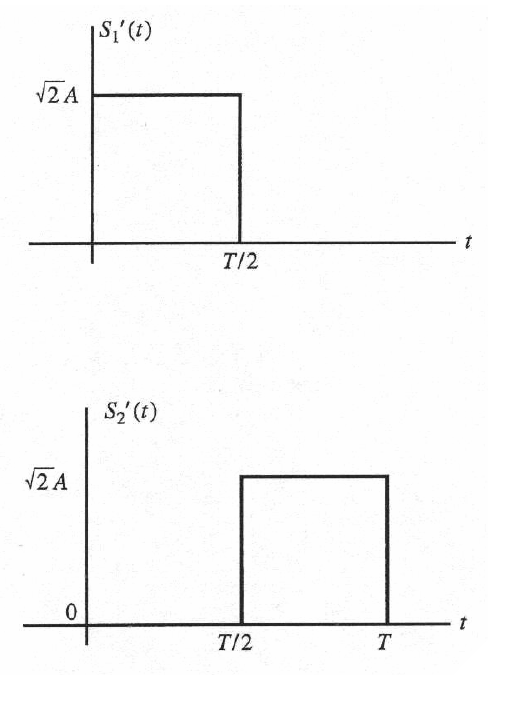
\includegraphics[scale = 1]{Due impulsi rettangolari che non si sovrappongono.PNG}
\end{figure}

La "filosofia" della PPM può essere generalizzata ad un numero di segnali maggiore di 2, 
e verrà ripresa in un paragrafo successivo riguardo agli spazi multi-dimensionali. \newline 

\newpage

\subsection{Segnali bi-ortogonali}
\footnote{Slide del prof | Formati di trasmissione numerica | pag 14 - 15\\  
Appunti di Damiano | pag 14 - 15\\
Slide | Formati di trasmissione numerica | pag  14 - 15\\
Appunti | 2025-03-28 | pag 8
}

Se ora si considera la seguente figura che abbiamo trovato precedentemente: 

\begin{figure}[h]
    \centering
    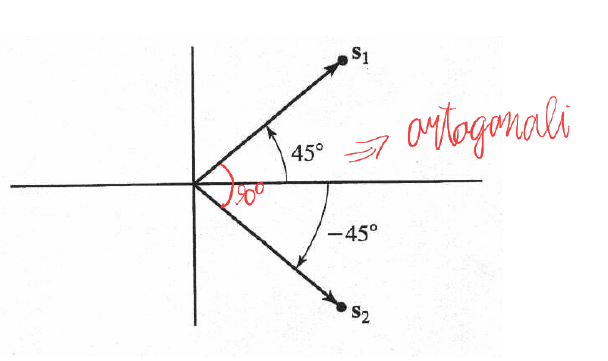
\includegraphics[scale = 1]{Piano bidimensionale dei coefficienti di Fourier in un piano N =2.PNG}
\end{figure}

e si considera i loro opposti, si può ottenere la seguente costellazione: 

\begin{figure}[h]
    \centering
    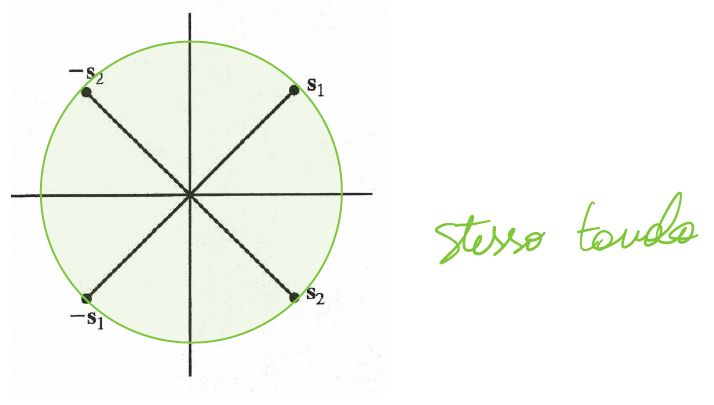
\includegraphics[scale = 1]{Costellazione con N = 2 e M = 4.PNG}
\end{figure}

cioè da M = 2, si ha una costellazione con M = 4. \newline 

\begin{tcolorbox}
Il concetto dei tavoli, del tavolo più grande e delle persone a tavola verrà spiegato successivamente. \newline

Un piccolo spoiler: non è detto che dovete andare all'IKEA a comprare un nuovo tavolo, ogni tanto si dovrà stare più stretti per far entrare tutti nello stesso tavolo.
\end{tcolorbox}

Quindi, rispetto al caso M = 2, nella costellazione con M = 4, i quattro segnali non sono più tra loro ortogonali. \newline 

Grazie alla scelta operata, questa tipo di costellazione definisce un insieme di forme d'onda decomponibile in due sottoinsieme, 
ciascuno di dimensione N = 2. \newline 

I segnali di ciascun sottoinsieme sono tra loro ortogonali, 
mentre i segnali di un sottoinsieme sono opposti a quelli dell'altro insieme. \newline 

Segnali con queste caratteristiche si dicono bi-ortogonali. \newline 

La loro generalizzazione verrà trattata successivamente. \newline 

Inoltre, in questo tipo di costellazione, con cioè M = 4, i segnali hanno la stessa energia e probabilità di errore di M = 2 perchè i segnali sono distribuiti nella stessa circonferenza. \newline

\newpage 

\subsection{Segnali nella stessa circonferenza}
\footnote{Slide del prof | Formati di trasmissione numerica | pag 15 \\  
Appunti di Damiano | pag 15 \\
Slide | Formati di trasmissione numerica | pag  15\\
Appunti | 2025-03-28 | pag 8
}

Ricordando che, con M = 4, questi segnali hanno la stessa energia perchè si trovano nella stessa circonferenza: 

\begin{figure}[h]
    \centering
    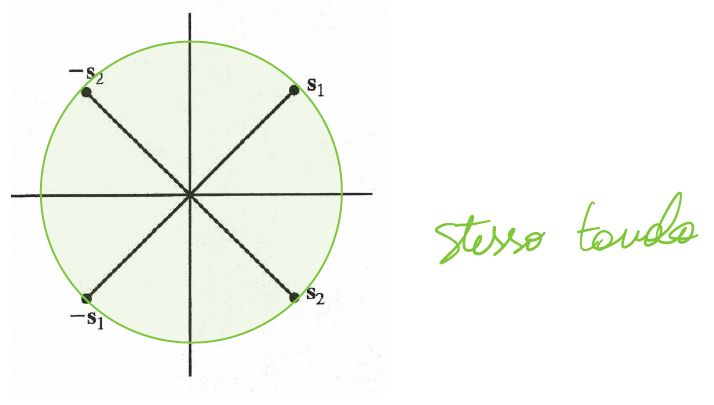
\includegraphics[scale = 1]{Costellazione con N = 2 e M = 4.PNG}
\end{figure}

allora possiamo aumentare gli M segnali e porli nella stessa circonferenza. \newline 

Considerando M = 8, possiamo avere questo caso: 

\begin{figure}[h]
    \centering
    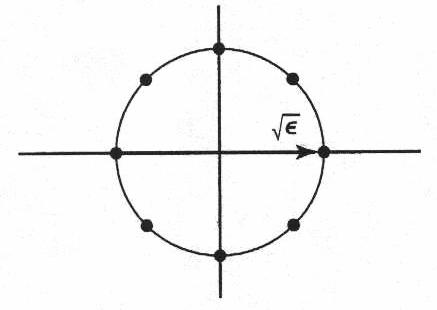
\includegraphics[scale = 1]{M = 8 stessa costellazione.png}
\end{figure}

Lasciando inalterato il raggio del cerchio, e dunque l'energia E, all'aumentare di M segnali, 
i punti rappresentativi dei segnali diventano sempre più vicini tra loro. \newline 

Posto infatti il vettore $\overrightarrow{s_m}$: 

{
    \Large 
    \begin{equation}
        \overrightarrow{s_m} 
        = 
        \left(\sqrt{E} \cdot \cos(\frac{2 \cdot \pi \cdot m}{M}), \sqrt{E} \cdot \sin(\frac{2 \cdot \pi \cdot m}{M})\right)
    \end{equation}
}

la radice quadrata della distanza Euclidea tra due punti della costellazione vale: 

{
    \Large 
    \begin{equation}
        \begin{split}
            d_{mn}
            &= 
            \sqrt{\abs{\overrightarrow{s_m} - \overrightarrow{s_n}}^{2}}
            \\
            &= 
            \dots 
            \\
            &= 
            \sqrt{2 \cdot E \cdot \left[ 1 - \cos(\frac{2 \cdot \pi \cdot (m - n)}{M})\right]}
        \end{split}
    \end{equation}
}

\begin{tcolorbox}
Da sottolineare, ma è anche inteso, che nella formula di $d_{mn}$ l'energia E è la stessa perchè i due punti si trovano nella stessa circonferenza   
\end{tcolorbox}

Se consideriamo: 

{
    \Large 
    \begin{equation}
        m - n = 1
    \end{equation}
}

consideriamo due punti adiacenti, 
in cui la distanza minima deve valere: 

{
    \Large 
    \begin{equation}
        d_{min}
        = 
        \sqrt{2 \cdot E \cdot \left[ 1 - \cos(\frac{2 \cdot \pi}{M})\right]}
    \end{equation}
}

\begin{tcolorbox}
    La distanza minima $d_{min}$ è il parametro più importante tra due punti perchè, 
    se la distanza minima non viene mantenuta, 
    il ricevitore interpreta un simbolo come un altro. \newline 

    Inoltre, dalla formula di $d_{min}$ si nota che, 
    se si vuole aumentare $d_{min}$, l'unico fattore che possiamo aumentare è l'energia E dei segnali 
\end{tcolorbox}

\newpage 

\subsection{Segnali in diverse circonferenze}
\footnote{Slide del prof | Formati di trasmissione numerica | pag 15 - 16\\  
Appunti di Damiano | pag 15 - 16\\
Slide | Formati di trasmissione numerica | pag  15 - 16\\
Appunti | 2025-03-28 | pag 8 \\
Appunti | 2025-03-31 | pag 2 \\
}

Rimuovendo il vincolo sull'energia, 
permettendo cioè che i segnali possano avere anche energie diverse tra loro, 
sono possibili altre costellazioni. \newline 

Due esempi, con M = 8, possiamo visualizzarlo di seguito (con le note): 

\begin{figure}[h]
    \centering
    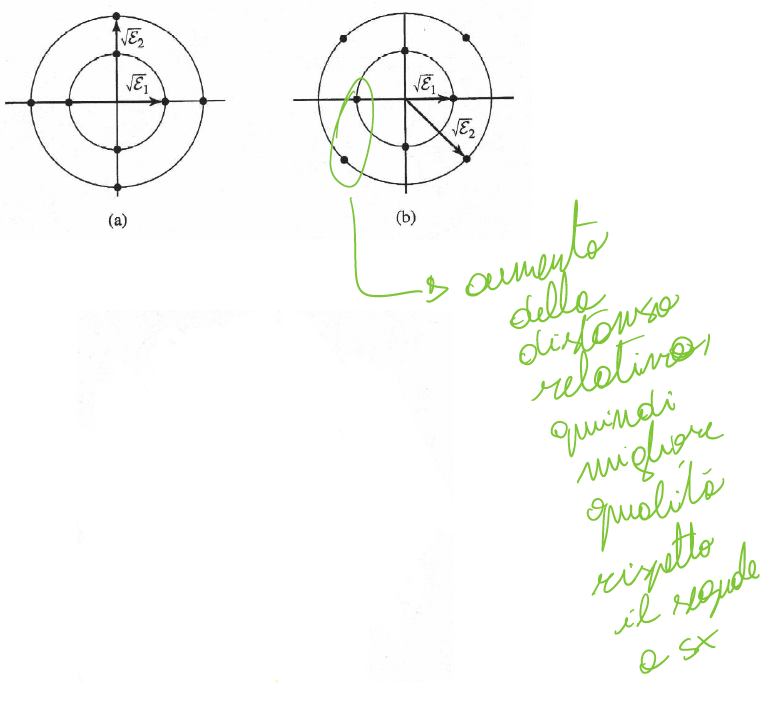
\includegraphics[scale = 1]{M = 8 ma con raggi diversi.PNG}
\end{figure}

In queste due esempi, i punti sono distribuiti su due cerchi (anziché uno come in precedenza) di raggio pari a $\sqrt{E_1}$ e $\sqrt{E_2}$, 
rispettivamente. \newline 

Qualitativamente, si può notare che la distanza minima per la costellazione (b) è maggiore rispetto alla distanza minima della costellazione (a). \newline 

Questo fatto risulta vantaggioso quando gli 8 segnali vengono utilizzati per la trasmissione dell'informazione in un sistema di telecomunicazione. \newline 

\newpage 

L'estensione di questa regola, cioè quella di aumentare l'energia per ogni circonferenza, 
la si può vedere in questo esempio in cui M = 16 : 

\begin{figure}[h]
    \centering
    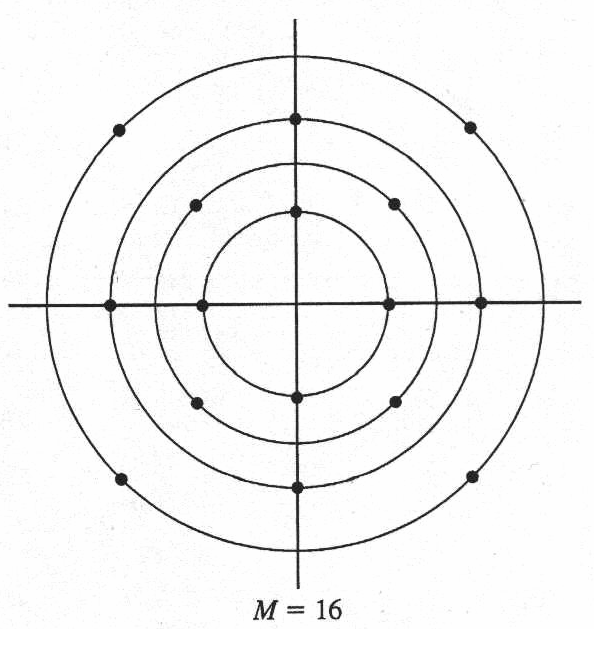
\includegraphics[scale = 0.6]{M = 16.png}
\end{figure}

\newpage 

\subsection{Costellazioni in segnali passa-banda}
\footnote{Slide del prof | Formati di trasmissione numerica | pag 16 - 17\\  
Appunti di Damiano | pag 16 - 17\\
Slide | Formati di trasmissione numerica | pag  16 - 17\\
Appunti | 2025-03-28 | pag 9 \\ 
Appunti | 2025-03-31 | pag 2 - 3 \\ 
}

Le costellazioni precedentemente studiate: 

\begin{figure}[h]
    \centering
    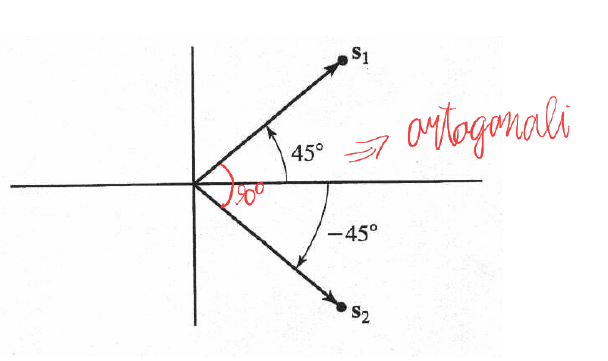
\includegraphics[scale = 0.5]{Piano bidimensionale dei coefficienti di Fourier in un piano N =2.PNG}
    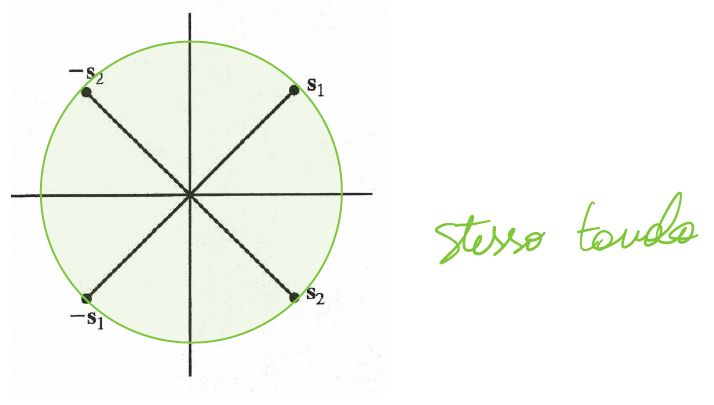
\includegraphics[scale = 0.5]{Costellazione con N = 2 e M = 4.PNG}
\end{figure}

riguardo ai segnali bi-ortogonali, 
sono segnali in banda base. \newline 

Questo tipo di costellazioni in banda base, possono essere estese al caso di rappresentazioni di segnali in passa banda utilizzando la relazione: 

{
    \Large 
    \begin{equation}
        u_m (t) 
        = 
        s_m (t)
        \cdot 
        \cos(2 \cdot \pi \cdot f_c \cdot t) 
        \text{ per } m = 1, 2, \dots, M \text{ e } 0 \le t \le T
    \end{equation}
}

dove $f_c$ è una opportuna frequenza di portante. \newline 

Se i segnali $s_m (t)$ (in cui m = 1, 2, $\dots$, M) hanno tutti la stessa energia E, cioè: 

{
    \Large 
    \begin{equation}
        E = \int_{0}^{T} \left[ s_{m} (t) \right]^{2} dt 
    \end{equation}
}

allora, anche i segnali $u_m (t)$ (in cui m = 1, 2, $\dots$, M) hanno, con buona approssimazione, tutti la stessa energia: 

{
    \Large 
    \begin{equation}
        \begin{split}
            E_s 
            &= 
            \int_{0}^{T}
            \left[ u_m (t)\right]^{2}
            dt
            \\
            &\approx
            \frac{1}{2}
            \cdot 
            \int_{0}^{T}
            \left[ s_m (t)\right]^{2}
        \end{split}
    \end{equation}
}

\begin{tcolorbox}
    Si è fatta questa approssimazione perchè, nella funzione integranda, 
    il termine oscillante, cioè $\cos(2 \pi f_c t)$, ipotizzando $f_c \textgreater \textgreater W$, 
    con banda W del segnale $s_m (t)$, dà un contributo trascurabile, se non, in certi casi, anche uguale a zero
\end{tcolorbox}

D'altro canto, ove lo spazio è bidimensionale sia rappresentativo di segnali passa-banda, 
le funzioni di base che generano lo spazio saranno sempre due. \newline 

In questo caso: 

{
    \Large 
    \begin{equation}
        \begin{cases}
            \Psi_1 (t) = \sqrt{\frac{2}{E_g}} \cdot g_T (t) \cdot \cos(2 \pi f_c t)
            \\
            \quad
            \\
            \Psi_2 (t) = \sqrt{\frac{2}{E_g}} \cdot g_T (t) \cdot \sin(2 \pi f_c t) 
        \end{cases}
    \end{equation}
}

dove $E_g$ è l'energia di $g_T (t)$. \newline 

\begin{tcolorbox}
    I termini sinusoidali nei termini delle funzioni di base, cioè $\cos(2 \pi f_c t)$ e $\sin(2 \pi f_c t)$, 
    rimarcano che non ci troviamo più in banda base, bensì in banda traslata
\end{tcolorbox}

Ove si assuma per $g_T (t)$ un impulso rettangolare, e cioè si pone: 

{
    \Large 
    \begin{equation}
        g_T (t) = \sqrt{\frac{2 \cdot E_s}{T}} \text{ per } 0 \le t \le T
    \end{equation}
}

la precedente si particolarizza come segue: 

{
    \Large 
    \begin{equation}
        \begin{split}
          u_m (t) 
        &= 
        s_m (t)
        \cdot 
        \cos(2 \cdot \pi \cdot f_c \cdot t) 
        \text{ per } m = 1, 2, \dots, M \text{ e } 0 \le t \le T
        \\
        &\downarrow
        \\
        u_m (t) 
        &= 
        \sqrt{\frac{2 \cdot E_s}{T}}
        \cdot 
        \cos(2 \cdot \pi \cdot f_c \cdot t + \frac{2 \pi m}{M}) 
        \text{ per } m = 0, 1, \dots, M - 1 \text{ e } 0 \le t \le T
        \end{split}
    \end{equation}
}

\begin{tcolorbox}
    Analizzando la nuova formula di $u_m (t)$, 
    la formula descrive l'andamento nel tempo di $u_m$. \newline 

    Dal punto di vista informativo, l'ampiezza $\sqrt{\frac{2 \cdot E_s}{T}}$ rimane costante, 
    quindi l'ampiezza non porta informazione. \newline 

    Il fattore che cambia nel tempo, e che porta informazione, 
    è $\cos(2 \cdot \pi \cdot f_c \cdot t + \frac{2 \pi m}{M}) $, 
    cioè la fase di $u_m (t)$
\end{tcolorbox}

Equivalentemente, 
utilizzando le funzioni di base, 
il generico segnale $\overrightarrow{u_m}$ è rappresentato dalle sue componenti: 

{
    \Large 
    \begin{equation}
        \overrightarrow{u_m}
        = 
        \left(
            \sqrt{E_s} \cdot \cos(\frac{2 \pi m}{M})
            , 
            \sqrt{E_s} \cdot \sin(\frac{2 \pi m}{M})
        \right)
    \end{equation}
}

dove $\overrightarrow{u_m}$ è un versore. \newline 

\newpage 

\subsubsection{Modulazioni con costellazioni di segnali passa-banda}
\footnote{Slide del prof | Formati di trasmissione numerica | pag 17 - 20\\  
Appunti di Damiano | pag 17 - 20\\
Slide | Formati di trasmissione numerica | pag  17 - 20\\
Appunti | 2025-03-28 | pag 9 \\ 
Appunti | 2025-03-31 | pag 3 - 5
}

Una trasmissione basata sull'invio di queste forme d'onda: 

{
    \Large 
    \begin{equation}
        \begin{split}
            E_m 
            &= 
            (s_m)^{2}
            \\
            &= 
            \left[ A_m \cdot \sqrt{E_g} \right]^{2}
            \\
            &= 
            A_m ^{2} \cdot E_g 
            \\
            &= 
            E_g \cdot A_m ^{2}   
        \end{split}
    \end{equation}
} 

utilizza la modulazione PSK (Phase Shift Keying). \newline 

La modulazione PSK definisce, quindi, un sistema di trasmissione in banda traslata, 
i cui segnali differiscono per la fase e sono caratterizzate dalla medesima energia. \newline 

Due forme d'onda adiacenti, differiscono per un angolo pari a $\frac{2 \pi}{M}$. \newline 

Per M = 2, la modulazione PSK, si riduce ad una modulazione 2-ASK introdotta in precedenza. \newline 

Un esempio di segnale 4-PSK (con le note) è mostrato di seguito: 

\begin{figure}[h]
    \centering
    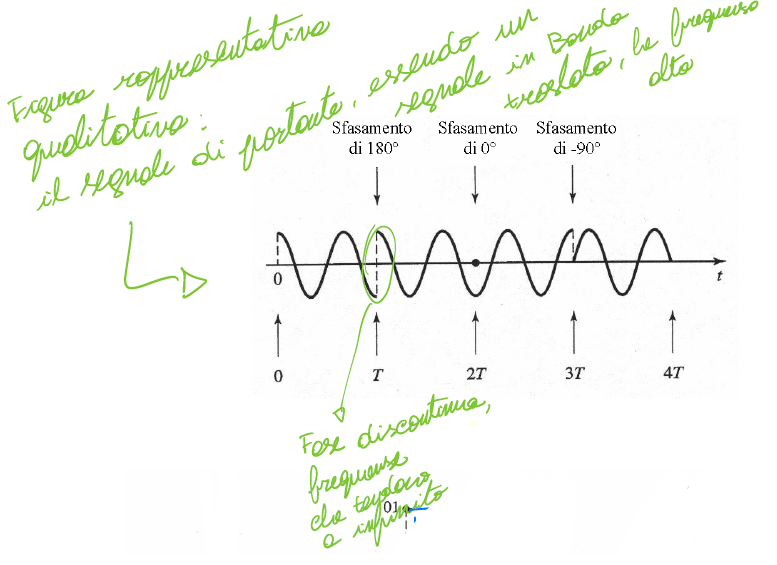
\includegraphics[scale = 1]{Esempio segnale 4-PSK.PNG}
\end{figure}

\newpage 

Un esempio di costellazioni per di PSK con M = 2, 4, 8 sono le seguenti figure: 

\begin{figure}[h]
    \centering
    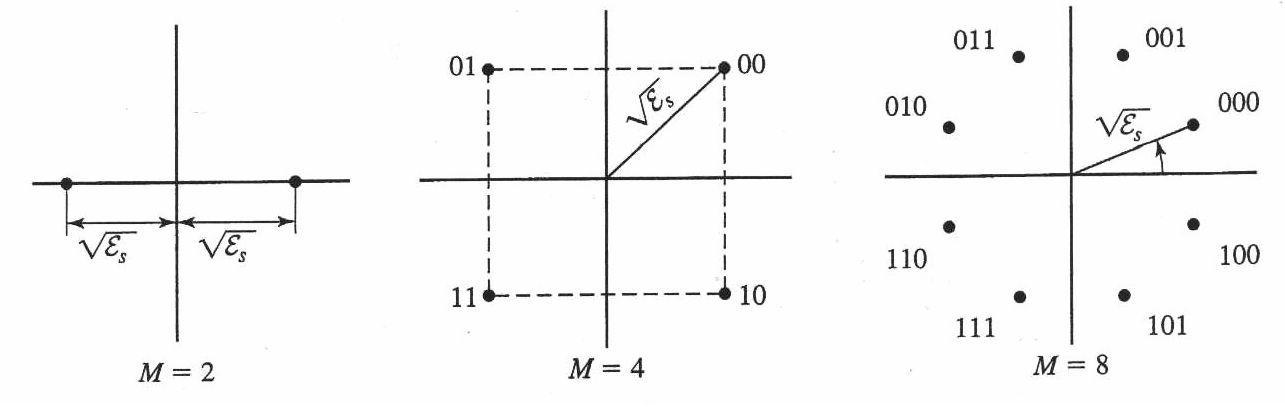
\includegraphics[scale = 0.7]{M-PSK Esempio costellazioni.png}
\end{figure}

Inoltre, queste figure ci permettono di mettere in evidenzia, 
per il caso M = 4 e M = 8, 
la possibilità di applicare la codifica di Gray. \newline 

Per codifica di Gray, si intende l'associazione bit a simboli (cioè mapping), 
la cui caratteristica peculiare è che sequenze binarie relative a simboli adiacenti differiscono di un solo bit 
(nota la codifica del singolo punto in binario). \newline 

Questa associazione, i.e. mapping, ha un enorme vantaggio per la qualità in trasmissione, 
perchè permette di minimizzare la probabilità di errore sul bit (o in breve BER: Bit Error Rate). \newline 

\begin{tcolorbox}
Possiamo ipotizzare che il rumore fa passare un segnale al suo punto adiacente. \newline 

Questo perchè, dal corso di Teoria dei Segnali, sappiamo che la probabilità del rumore termico è di tipo gaussiano, 
cioè che il rumore impatta di più sui valori più piccoli rispetto ai valori più alti. \newline 

In questo caso, il rumore termico impatta di più sull'LSB (Least Significant Bit), cioè il bit più piccolo, 
che, grazie alla codifica di Gray, fa al massimo muovere il segnale da punto desiderata a quello adiacente. \newline 

Inoltre, la codifica di Gray è efficace nelle modulazioni in cui i simboli sono equiprobabili. 
\end{tcolorbox}

Sempre nel caso di modulazioni in banda traslata, 
la rimozione del vincolo sull'energia (presente nel formato PSK), 
conduce alla definizione della QAM (Quadrature Amplitude Modulation). \newline 

\begin{tcolorbox}
    La QAM è LA modulazione che letteralmente utilizzi tutti i giorni, perchè viene implementata dallo standard WiFi (e non solo). \newline 

    Ti lascio un po' di video sulla spiegazione della QAM: \newline 

    \url{https://www.youtube.com/watch?v=xn9zqSoOlcE&t=20s}\\
    Wireless Communication - Eight: Quadrature Amplitude Modulation by Computer Science Lessons \newline 

    La QAM viene impiegato anche nello standard 5G, e quindi anche dai modem contenuti nei chipset dei nostri cellulari: \newline 

    \url{https://www.youtube.com/watch?v=iEWUWTfVGqI} \\
    Snapdragon 888: la vera novità per la connettività è la carrier aggregation 5G! by Stefano Bolis
\end{tcolorbox}

Ferma restando la rappresentazione su uno spazio bidimensionale (cioè N = 2), 
i simboli QAM sono distribuiti in modo da non trovarsi, necessariamente, alla stessa distanza dall'origine. \newline 

Questo corrisponde ad aumentare il numero dei gradi di libertà di sistema, per cui la generica forma d'onda trasmessa potrà scriversi: 

{
    \Large 
    \begin{equation}
        u_{mn}
        = 
        A_m \cdot g_T (t) \cos(2 \pi f_c t + \theta_n) \text{ per } m = 1, 2, \dots, M_1 \text{ , } n = 1, 2, \dots, M_2
    \end{equation}
}

I vari segnali differiscono quindi per la fase (come nel sistema PSK), 
ma anche per l'ampiezza e M sarà uguale: 

{
    \Large 
    \begin{equation}
        M = M_1 \cdot M_2
    \end{equation}
}

Esempi classici della QAM, qui per M = 16, è riportata di seguito: 

\begin{figure}[h]
    \centering
    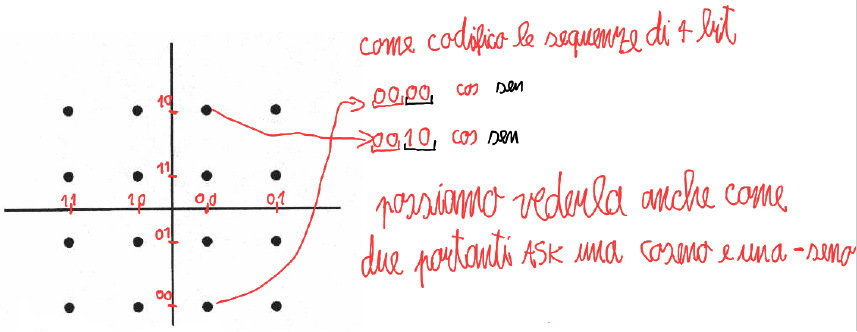
\includegraphics[scale = 1]{16 - QAM con note.PNG}
\end{figure}

\begin{tcolorbox}
La 16-QAM assomiglia alla PSK, alche con la PSK hanno in comune le stesse funzioni di base    
\end{tcolorbox}

Invece, con la seguente figura, possiamo confrontare tutte le possibili costellazioni di QAM dalla M = 4 alla M = 64 (con note): 

\begin{figure}[h]
    \centering
    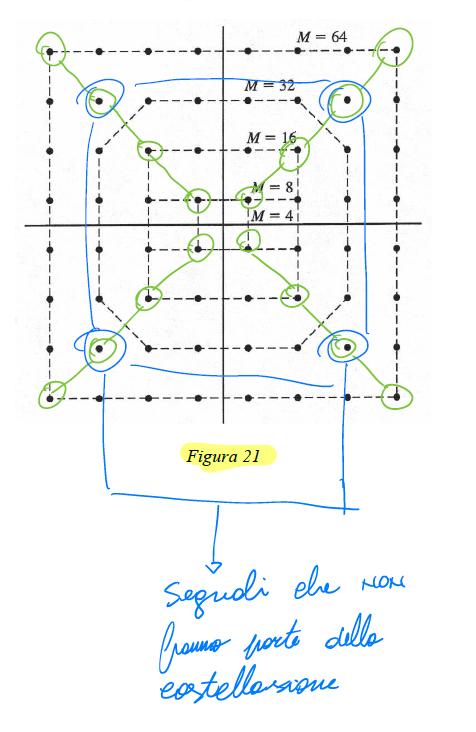
\includegraphics[scale = 0.8]{Dalla 4-QAM alla 64-QAM costellazioni.PNG}
\end{figure}

Le costellazione nel caso di: 

{
    \Large
    \begin{equation}
        M = 2^{k}
    \end{equation}
}

dove k è un numero pari, formano costellazioni che sono quadrati perfetti (si può notare la costellazione di M = 4, o M = 64). \newline 

Invece le costellazioni con k dispari maggiore di 3, ad esempio M = 32, 
formano una costellazione a croce (in inglese cross-constellation), 
formando una costellazione di un quadrato perfetto senza i punti degli angoli. \newline 

\begin{tcolorbox}
    Proprio per questo motivo, generalmente viene utilizzando un M in cui k è pari. \newline 

    Ricordiamo che, se possibile, specialmente nel campo Wireless, bisogna utilizzare tutto quello che si ha per migliorare la qualità della trasmissione e la sua efficienza. \newline 

    Un detto popolare dice "Del porco, non si butta via nulla": anche nel campo delle telecomunicazioni, se possibile, non bisogna buttare via nulla. \newline 

    "Buttare" dei simboli è "un privilegio" certe volte. 
\end{tcolorbox}

Lo schema di un demodulatore è il seguente: 

\begin{figure}[h]
    \centering
    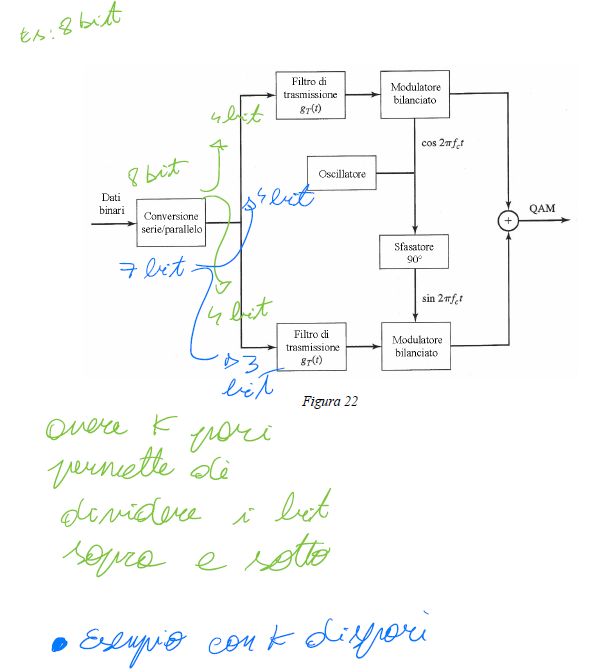
\includegraphics[scale = 1.3]{QAM modulatore schema.PNG}
\end{figure}

Le due portanti, sfasate di $90^{\circ}$ definiscono lo spazio bidimensionale. \newline 

La conversione serie-parallelo separa i bit che selezioneranno l'ampiezza di ciascuna delle due portanti in quadratura, in accordo con la costellazione specificata. \newline 


\begin{tcolorbox}
    Ricordiamo anche l'implicazione di avere un M elevato: l'aumento della banda in frequenza. \newline 

    Certe volte può essere un vantaggio (si pensi alla 4096-QAM del Wifi 7 con il quale si possono trasmettere un flusso teorici di 40 Gbps con 320 MHz di banda), 
    ma altre volte uno svantaggio (si pensi ad un operatore di rete telefonica che paga per la banda e deve inserire più utenti contemporaneamente). \newline 

    Un po' di link per avere una panoramica sulle implicazioni che esistono realmente ad oggi giorno: \newline 

    \url{https://www.qualcomm.com/content/dam/qcomm-martech/dm-assets/documents/Qualcomm-Wi-Fi-7-Reference-Guide.pdf} \newline 

    \url{https://www.youtube.com/watch?v=Db4RcNPIDVU} \\
    Il 5G ha problemi di velocità e copertura in upload: cause e soluzioni! by Stefano Bolis \newline 

    \url{https://www.youtube.com/watch?v=mSO0PbBt9hs} \\
    Frequenze 5G in banda C: gli operatori italiani le hanno pagate il doppio! by Stefano Bolis 

\end{tcolorbox}

\newpage 

\section{Segnali ortogonali, transagonali e bi-ortogonali}
\footnote{Slide del prof | Formati di trasmissione numerica | pag 21 \\  
Appunti di Damiano | pag 21 \\
Slide | Formati di trasmissione numerica | pag  21\\
Appunti | 2025-03-31 | pag 6 
}

Già nel paragrafo precedente si sono forniti esempi di segnali ortogonali, 
e sono state date informazioni in merito alla loro rappresentazione, 
ma limitatamente al caso bi-dimensione. \newline 

In realtà, la proprietà di ortogonalità può essere estesa ad un insieme di segnali di dimensione arbitraria, 
ciascuno, ad esempio, di durata T. \newline 

Di seguito due esempi di segnali con M = 4 (con note): 

\begin{figure}[h]
    \centering
    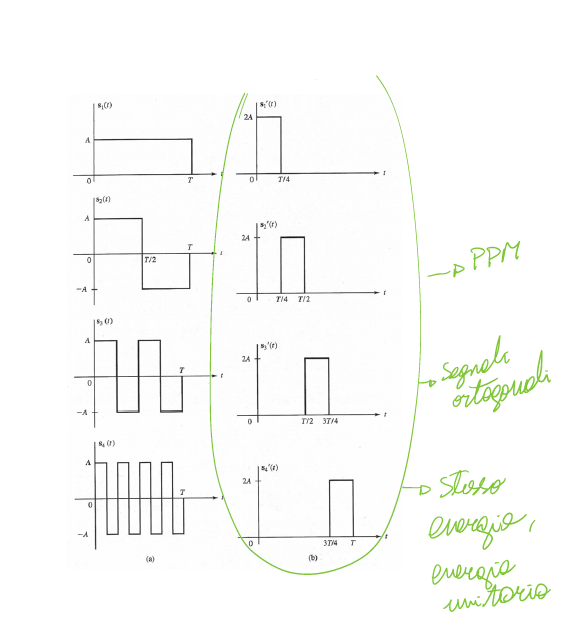
\includegraphics[scale = 1.4]{4-PPM segnali.PNG}
\end{figure} 

A destra un sistema diverso da quello a sinistra. \newline 

L'implementazione della ortogonalità tra i vari segnali, 
con i due sistemi, è diversa. \newline 

Ricordiamo la definizione di ortogonalità tra due segnali: 

{
    \Large 
    \begin{equation}
        \int 
        s_1 (t) \cdot s_2^{*} (t) dt 
        = 
        0
    \end{equation}
}

dove: 

\begin{itemize}
    \item si pone gli estremi di integrazione dell'integrale nei tratti in cui si vuole calcolare la ortogonalità tra $s_1 (t)$ e $s_2 (t)$ 
    \item per $s_2^{*} (t)$ si intende il coniugato di $s_2(t)$
\end{itemize}

L'ortogonalità dei segnali a sinistra, cioè i segnali [$s_1 (t), s_2 (t), s_3 (t), s_4 (t)$], 
sono tutti diversi da zero nell'intervallo $[0, T]$. \newline 

In questo caso, l'ortogonalità viene conseguita attraverso una oculata assegnazione di sotto-intervalli, 
in cui le funzioni valgono, alternativamente +A e -A. \newline 

Invece, nel sistema a destra, cioè i segnali [$s_1^{'} (t), s_2^{'} (t), s_3^{'} (t), s_4^{'} (t)$], 
sono ottenuti con un unico impulso di durata $\frac{T}{4}$, che, nei vari segnali, viene traslato in periodi di $\frac{T}{4}$. \newline 

Ciò, garantisce una facile implementazione dell'ortogonalità tra i segnali e inoltre, 
nello stesso intervallo multiplo di $\frac{T}{4}$, i vari segnali non si sovrappongono: 
questa classe di segnali, generalizzata a un valore M qualsiasi, 
prende il nome di PPM (Pulse Position Modulation). \newline 

\begin{tcolorbox}
    Grazie alla sua facilità di implementazione, la PPM è molto usata nel campo della fibra ottica, perchè impulso alto significa luce del laser, no impulso significa laser spento. \newline 

    Delle letture sull'implementazione reale della PPM: \newline 

    \url{https://ieeexplore.ieee.org/document/5637976} \\
    Pulse position modulation (PPM) fiber optic architectures \newline 

    \url{https://ntrs.nasa.gov/api/citations/19680025702/downloads/19680025702.pdf} \\
    The design of a Pulse Position Modulated (PPM) Optical Communication System 

\end{tcolorbox}

\newpage 

\subsection{PPM (Pulse Position Modulation)}
\footnote{Slide del prof | Formati di trasmissione numerica | pag 21 - 22\\  
Appunti di Damiano | pag 21 - 22\\
Slide | Formati di trasmissione numerica | pag  21 - 22\\
Appunti | 2025-03-31 | pag 6
}

La PPM viene chiamata Pulse Position Modulation proprio in ragione del fatto che i vari segnali sono discriminati sulla base della posizione di un impulso 
(che nel caso generale avrà durata $\frac{T}{M}$). \newline 

Tutti i segnali visti nella figura dei due sistemi in cui i segnali sono ortogonali tra di loro:

\begin{figure}[h]
    \centering
    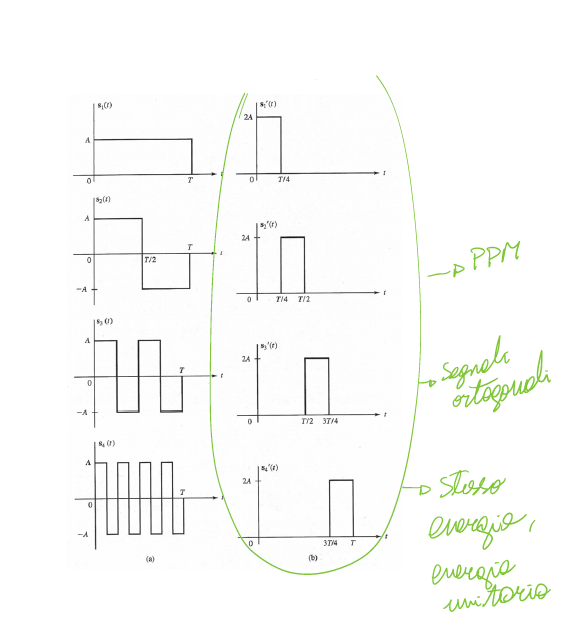
\includegraphics[scale = 0.8]{4-PPM segnali.PNG}
\end{figure} 

hanno la stessa energia E, che vale: 

{
    \Large 
    \begin{equation}
        E = A^{2} \cdot T
    \end{equation}
}

Per rappresentare l'insieme di M forme d'onda ortogonali, 
è necessario uno spazio di dimensione: 

{
    \Large 
    \begin{equation}
        N = M = 4
    \end{equation}
}

Quindi, su questo spazio, gli M segnali sono rappresentati dai vettori con i seguenti componenti: 

{
    \Large 
    \begin{equation}
        \begin{cases}
        \overrightarrow{s_1} = \left( \sqrt{E}, 0, 0, \dots, 0 \right)  
        \\
        \overrightarrow{s_2} = \left( 0 , \sqrt{E}, 0, \dots, 0 \right)  
        \\
        \dots
        \\
        \overrightarrow{s_M} = \left( 0 , 0, 0, \dots, \sqrt{E} \right)  
        \end{cases}
    \end{equation}
}

\begin{tcolorbox}
    Come abbiamo studiato ad Algebra Lineare, 
    per noi la M dimensione sarà o un vettore o una matrice
\end{tcolorbox}

\newpage 

\subsubsection{PPM con base di impulsi rettangolari}
\footnote{Slide del prof | Formati di trasmissione numerica | pag 22 \\  
Appunti di Damiano | pag 22 \\
Slide | Formati di trasmissione numerica | pag  22\\
Appunti | 2025-03-31 | pag 6
}

Siccome l'uomo non può concepire e visualizzare la M-dimensione, cioè oltre alla terza in poi, 
concentriamoci al caso M = 3, cioè al caso tridimensionale. \newline 

Rappresentando in una figura vettoriale, possiamo rappresentare le basi di una 3-PPM con questa figura: 

\begin{figure}[h]
    \centering
    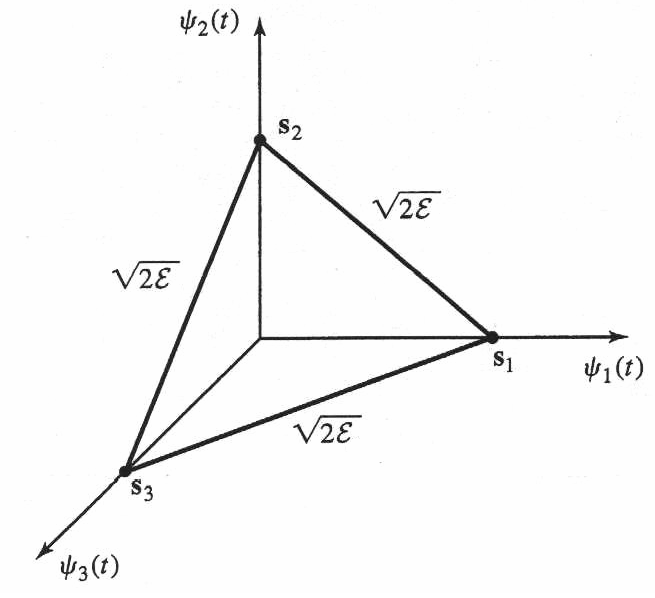
\includegraphics[scale = 0.8]{3-PPM Basi.png}
\end{figure} 

Ritornando al caso generale in cui M può essere un qualsiasi numero intero, l
e funzioni di base nel caso PPM sono: 

{
    \Large 
    \begin{equation}
        \Psi_m (t)
        = 
        \begin{cases}
            \frac{1}{\sqrt{E_g}}
            \cdot 
            g \left[ t - \frac{(m-1) \cdot T}{M}\right]
            \text{ per }
            \frac{(m-1) \cdot T}{M} \le t \le \frac{m \cdot T}{M}
            \\
            \quad
            \\
            0 \text{ altrove}
        \end{cases}
    \end{equation}
}

dove $g_T (t)$ è una funzione arbitraria (nel caso della PPM, abbiamo scelto come funzione arbitraria l'impulso rettangolare). \newline 

La radice quadrata della distanza Euclidea tra due segnali è la stessa per tutte le coppia di segnali e vale:

{
    \Large 
    \begin{equation}
        \begin{split}
            d_{mn}
            &= 
            \sqrt{\abs{\overrightarrow{s_m} - \overrightarrow{s_n}}^{2}}
            \\
            &= 
            \dots
            \\
            &= 
            \sqrt{2 \cdot E}
        \end{split}
    \end{equation}
}

\newpage 

\subsection{FSK (Frequency Shift Keying)}
\footnote{Slide del prof | Formati di trasmissione numerica | pag 22 - 24\\  
Appunti di Damiano | pag 22 - 24\\
Slide | Formati di trasmissione numerica | pag  22 - 24\\
Appunti | 2025-03-31 | pag 6 - 8 \\
Appunti | 2025-04-01 | pag 2 \\
Appunti | 2025-07-21 Ricevimento| pag 5.1
}

L'ortogonalità dei segnali, ad esempio quelli che abbiamo visto nella figura della 4-PPM, 
viene ottenuta ragionando nel dominio del tempo. \newline 

Equivalentemente, i segnali ortogonali possono essere ottenuti anche ragionando nel dominio della frequenza. \newline 

Consideriamo, ad esempio, i seguenti segnali: 

{
    \Large 
    \begin{equation}
        \begin{cases}
            u_1 (t) = \sqrt{\frac{2 \cdot E}{T}} \cos(2 \pi f_1 t)
            \\
            u_2 (t) = \sqrt{\frac{2 \cdot E}{T}} \cos(2 \pi f_2 t)
        \end{cases}
    \end{equation}
}

queste equazioni valgono solo per $0 \le t \le T$. \newline 

Dal punto di vista informativo, $u_1 (t)$ e $u_2 (t)$ hanno la stesa ampiezza, 
che è $\sqrt{\frac{2 \cdot E}{T}}$, 
ciò che varia nel tempo è la fase perchè hanno $\cos(2 \pi f_1 t)$. \newline 

Inoltre, in questi segnali: 

{
    \Large 
    \begin{equation}
        f_1 \neq f_2
    \end{equation}
}

quindi, in fase di progettazione del sistema, le frequenze sono due gradi di libertà. \newline 

La frequenza di portante $f_c$ e la differenza tra le due frequenze, sarà uguale a: 

{
    \Large 
    \begin{equation}
        \begin{cases}
            f_c = \frac{f_1 + f_2}{2}
            \\
            \quad
            \\
            \Delta f = f_2 - f_1
        \end{cases}
    \end{equation}
}

Alla fine di tutte queste osservazioni, 
possiamo concludere che $u_1 (t)$ e $u_2 (t)$ sono due funzioni oscillanti, 
con durata limitata all'intervallo $[0, T]$ a frequenza diversa. \newline 

Il segnale prende il nome di FSK (Frequency Shift Keying). \newline 

\newpage 

Di seguito l'andamento nel tempo di un segnale 2-FSK: 

\begin{figure}[h]
    \centering
    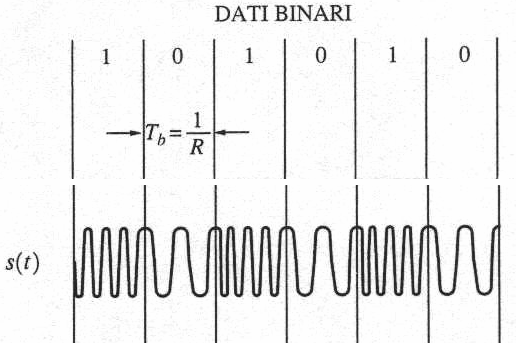
\includegraphics[scale = 0.8]{2-FSK andamento nel tempo di segnale nel tempo.png}
\end{figure}

Invece, l'andamento nel tempo (normalizzato nel periodo T) di un segnale 4-FSK: 

\begin{figure}[h]
    \centering
    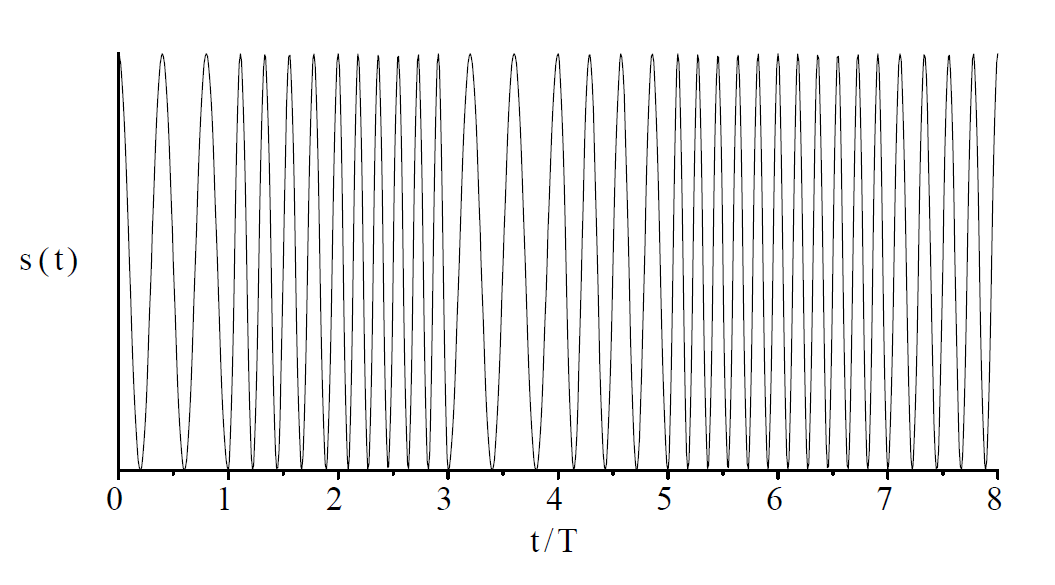
\includegraphics[scale = 0.6]{4-FSK andamento nel tempo di segnale nel tempo.png}
\end{figure}

quindi nella 4-FSK ci saranno 4 frequenze differenti. \newline 

Tornando alla 2-FSK, posto: 

{
    \Large 
    \begin{equation}
        f_2 = f_1 + \Delta f
    \end{equation}
}

il problema si traduce, evidentemente, nella scelta del valore di $\Delta f$. \newline 

\newpage 

Si può calcolare il coefficiente di correlazione che, 
nel caso di segnali con (approssimativamente) la stessa energia, quali quelli in esame, è così definito: 

{
    \Large 
    \begin{equation}
        \gamma_{12}
        =
        \frac
        {
        \int_{0}^{T_b}
        u_1 (t) \cdot u_2 (t) dt 
        }{E_b}
    \end{equation}
}

\begin{tcolorbox}

    Il coefficiente di correlazione $\gamma_{12}$ è un coefficiente di qualità. \newline 

    I calcoli sono stati svolti considerando le due frequenze $f_1$ e $f_2$ molto vicini, 
    così da considerare un basso su $\Delta f$ dato dal rumore. \newline 

    $\gamma_{12}$ può assumere diversi valori, in base alle caratteristiche dei segnali $u_1 (t)$ e $u_2 (t)$. \newline 
    
    Se: 
{
    \Large 
    \begin{equation}
     \gamma_{12} = -1   
    \end{equation}
}
   allora: 
   
   {
    \Large 
    \begin{equation}
     u_2 (t) = -u_1 (t)   
    \end{equation}
   }

    i segnali sono opposti, cioè anti-podali, 
    e non sono ortogonali come nel caso della  2-PAM
\end{tcolorbox}

$\gamma_{12}$ rispetto a $\Delta f$ ha questo tipo di andamento (con note): 

\begin{figure}[h]
    \centering
    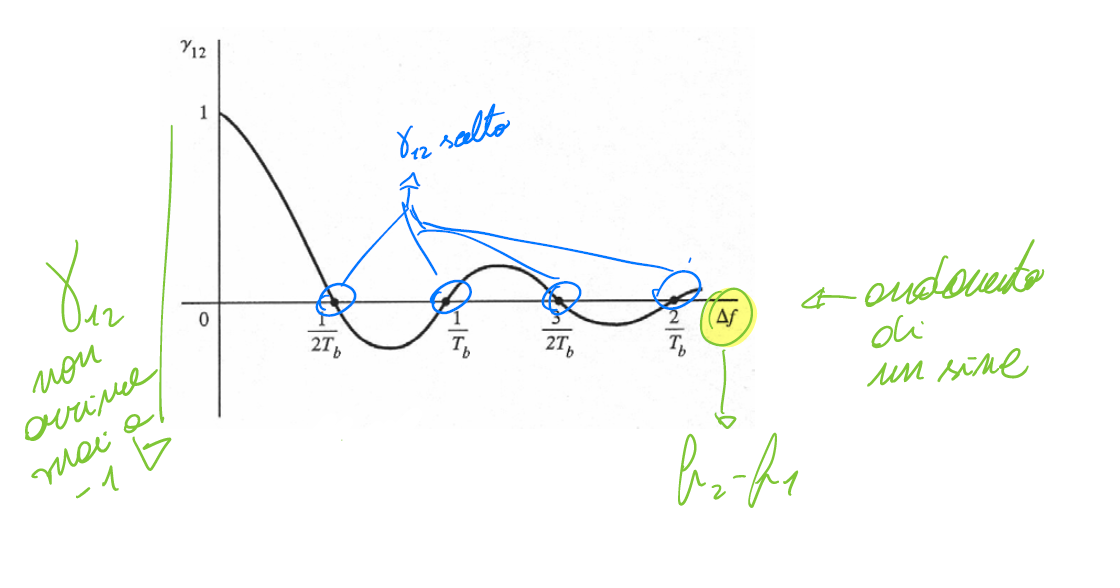
\includegraphics[scale = 0.8]{Coefficiente di correlazione rispetto alla differenza di frequenza nella 2-FSK.PNG}
\end{figure}

Dalla figura, si nota che per: 

{
    \Large 
    \begin{equation}
        \Delta f = \frac{1}{2 \cdot T_b}
    \end{equation}
}

e suoi multipli, 
il coefficiente di correlazione $\gamma_{12}$ si annulla perchè le due forme d'onda sono tra loro ortogonali. \newline 

\begin{tcolorbox}

$u_2 (t)$ si intende il suo coniugato come nel caso di calcolo dell'integrale per capire se due segnali sono ortogonali
\end{tcolorbox}

D'altro canto, 
è anche possibile verificare che questo risultato, cioè la formula di $u_1 (t)$ e $u_2 (t)$: 

{
    \Large 
    \begin{equation}
        \begin{cases}
            u_1 (t) = \sqrt{\frac{2 \cdot E}{T}} \cos(2 \pi f_1 t)
            \\
            u_2 (t) = \sqrt{\frac{2 \cdot E}{T}} \cos(2 \pi f_2 t)
        \end{cases}
    \end{equation}
}

è valido sotto l'ipotesi che le due forme d'onda $u_1 (t)$ e $u_2 (t)$ abbiano identica fase iniziale (che per semplicità consideriamo nulla). \newline 

Se la fase iniziale non è nulla, e quindi possiamo scrivere $u_2 (t)$ come: 

{
    \Large 
    \begin{equation}
        u_2 (t) = \sqrt{\frac{2 \cdot E_b}{T_b}} \cdot \cos(2 \pi f_2 t + \Delta \phi) 
        \text{ per } 0 \le t \le T_b
    \end{equation}
}

dove $\Delta \phi$ è la differenza di fase tra $u_1 (t)$ e $u_2 (t)$, 
allora la condizione di ortogonalità sarebbe comunque verificato, 
indipendentemente dal valore di $\Delta \phi$, 
assumendo però: 

{
    \Large 
    \begin{equation}
        \Delta f 
        =
        \frac{1}{T_b}
    \end{equation}
}

\begin{tcolorbox}
    Controllare la fase dei segnali in un sistema di telecomunicazioni è molto complicato, 
    perchè, come abbiamo visto nelle modulazioni angolari, il rumore può impattare tanto la ricezione. \newline 

    Inoltre, il recupero della fase di un segnale va svolto con diversi componenti, 
    tra cui il PLL, elemento complesso e difficile da implementare perchè aumenta un costo economico al ricevitore e un costo di tempo computazionale. \newline 

    Più ci semplifichiamo il ricevitore, e il sistema tutto, e meglio è per tutti.
\end{tcolorbox}

Inoltre, la figura dell'andamento di $\gamma_{12}$ mette anche in evidenzia che si può conseguire un valore del coefficiente di correlazione 
anche più "favorevole" (dal punto di vista della differenziazione delle forme d'onda), 
assumendo un valore di $\Delta f$ uguale a: 

{
    \Large 
    \begin{equation}
        \Delta f = 
        \frac{0.715}{T_b} 
    \end{equation}
}

avremo un valore di $\gamma_{12}$ uguale a: 

{
    \Large 
    \begin{equation}
        \gamma_{12} = -0.217
    \end{equation}
}

valore che è "più vicino" a $\gamma_{12} = -1$ (anche se è molto lontano), 
e che quindi, come abbiamo visto nella 2-PSK, garantisce una distanza tra i due punti massima. \newline 

Ma questo valore $\gamma_{12}$ è difficile da gestire, quindi si sceglie di utilizzare $\gamma_{12} = 0$ 
perchè i segnali da generare sono ortogonali, quindi semplici da generare. \newline 

Quindi, l'ortogonalità è sempre verificata nella 2-FSK se: 

{
    \Large 
    \begin{equation}
        \Delta f = \frac{k}{2 \cdot T_b}
    \end{equation}
}

con k numero intero. \newline 

Generalmente si assume: 

{
    \Large 
    \begin{equation}
        k = 1
    \end{equation}
}

perchè permette di minimizzare l'occupazione spettrale. \newline 

\newpage 

\subsection{Forme d'onda bi-ortogonali}
\footnote{Slide del prof | Formati di trasmissione numerica | pag 24 - 25\\  
Appunti di Damiano | pag 24 - 25\\
Slide | Formati di trasmissione numerica | pag  24 - 25\\
Appunti | 2025-04-01 | pag 2
}

A partire da un insieme di forme d'onda ortogonali, 
è possibile costruire un insieme di forme d'onda bi-ortogonali. \newline 

Un esempio di forme bi-ortogonali lo avevo già visto in precedenza: 

\begin{figure}[h]
    \centering
    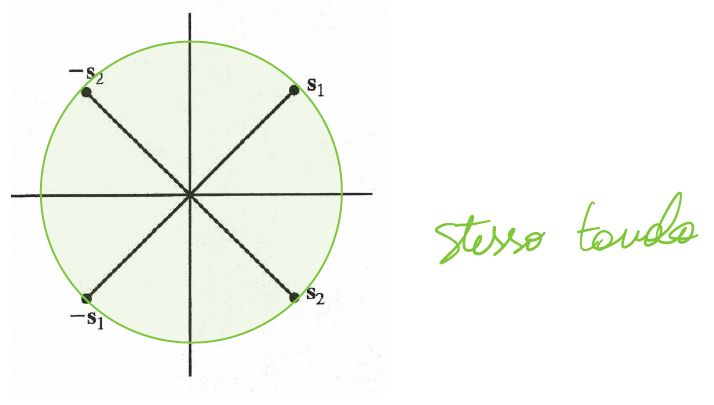
\includegraphics[scale = 0.5]{Costellazione con N = 2 e M = 4.PNG}
\end{figure}

Considerando M segnali, 
a partire dall'insieme ortogonale, 
si considera l'insieme delle forme d'onda opposte (sfasate cioè di $180^{\circ}$). \newline 

In tal modo, le M forme d'onda sono divise in due gruppi di $\frac{M}{2}$ forme d'onda. \newline 

All'interno di ciascun gruppo, 
le forme d'onda sono ortogonali. \newline 

Le forme d'onda di un gruppo sono, poi, opposte alle forme d'onda dell'altro gruppo. \newline 

Stanti le peculiarità dell'insieme, 
la dimensione dello spazio in cui sono rappresentati i segnali vale: 

{
    \Large 
    \begin{equation}
        N = \frac{M}{2}
    \end{equation}
}

I vettori rappresentativi degli M segnali, avranno dunque $\frac{M}{2}$ componenti e saranno esprimibili come: 
{
    \Large 
    \begin{equation}
        \begin{cases}
        \overrightarrow{s_1} = \left( \sqrt{E}, 0, 0, \dots, 0 \right)  
        \\
        \overrightarrow{s_2} = \left( 0 , \sqrt{E}, 0, \dots, 0 \right)  
        \\
        \dots
        \\
        \overrightarrow{s_{\frac{M}{2}}} = \left( 0 , 0, 0, \dots, \sqrt{E} \right)  
        \\
        \overrightarrow{s_{\frac{M}{2} + 1}} = \left( - \sqrt{E}, 0, 0, \dots, 0 \right)  
        \\
        \dots
        \\
        \overrightarrow{s_{M}} = \left( 0 , 0, 0, \dots, - \sqrt{E} \right)  
    \end{cases}
    \end{equation}
}

Quindi l'insieme dei vettori N $[\overrightarrow{s_1}, \overrightarrow{s_2}, \dots, \overrightarrow{s_{\frac{M}{2}}} ]$ 
forma la base dello spazio M. \newline 

L'insieme dei vettori $[\overrightarrow{s_{\frac{M}{2} + 1}}, \dots, \overrightarrow{s_{M}}]$ 
sono opposti ai vettori della base, 
cioè sono opposti ai vettori $[\overrightarrow{s_1}, \overrightarrow{s_2}, \dots, \overrightarrow{s_{\frac{M}{2}}} ]$. \newline 

\newpage 

\subsection{Forme d'onda transagonali}
\footnote{Slide del prof | Formati di trasmissione numerica | pag 25 \\  
Appunti di Damiano | pag 25 \\
Slide | Formati di trasmissione numerica | pag  25\\
Appunti | 2025-04-01 | pag 2
}

Accanto ai concetti di ortogonalità e bi-ortogonalità, 
può essere introdotto anche il concetto di trasortogonalità. \newline 

Estendendo la definizione di coefficiente di correlazione $\gamma_{mn}$ visto precedentemente per segnali $u_1 (t)$ e $u_2 (t)$ con la stessa energia $E_b$, 
possiamo estenderlo a due segnali $s_m (t)$ e $s_n (t)$ aventi rispettivamente energie $E_m$ e $E_n$. \newline 

Quindi la formula del coefficiente di correlazione diventerà:

{
    \Large 
    \begin{equation}
        \begin{split}
        \gamma_{12}
        &=
        \frac
        {
        \int_{0}^{T_b}
        u_1 (t) \cdot u_2 (t) dt 
        }{E_b}
        \\
        &\downarrow
        \\
        \gamma_{mn}
        &=
        \frac
        {
        \int_{0}^{T}
        s_m (t) \cdot s_n (t) dt 
        }{\sqrt{E_m \cdot E_n}}
        \end{split}
    \end{equation}
}

Per segnali ortogonali, 
il coefficiente di correlazione è nullo (perchè l'integrale è nullo). \newline 

Se abbiamo delle forme d'onda che hanno la stessa energia: 

{
    \Large 
    \begin{equation}
        E_m = E_n = E
    \end{equation}
}

allora, la formula del coefficiente di correlazione diventa: 

{
    \Large 
    \begin{equation}
     \gamma_{mn}
        =
        \frac
        {
        \int_{0}^{T}
        s_m (t) \cdot s_n (t) dt 
        }{E}   
    \end{equation}
}

e si verifica che (cioè non lo dimostriamo) 
se lo spazio è formato da vettori bi-ortogonali: 

{
    \Large 
    \begin{equation}
        \begin{cases}
        \overrightarrow{s_1} = \left( \sqrt{E}, 0, 0, \dots, 0 \right)  
        \\
        \overrightarrow{s_2} = \left( 0 , \sqrt{E}, 0, \dots, 0 \right)  
        \\
        \dots
        \\
        \overrightarrow{s_{\frac{M}{2}}} = \left( 0 , 0, 0, \dots, \sqrt{E} \right)  
        \\
        \overrightarrow{s_{\frac{M}{2} + 1}} = \left( - \sqrt{E}, 0, 0, \dots, 0 \right)  
        \\
        \dots
        \\
        \overrightarrow{s_{M}} = \left( 0 , 0, 0, \dots, - \sqrt{E} \right)  
    \end{cases}
    \end{equation}
}

il minimo valore di $\gamma_{mn}$ (in modulo e segno) è: 

{
    \Large 
    \begin{equation}
        \gamma_{mn} = - \frac{1}{M - 1}
    \end{equation}
}

Forme d'onda con questa caratteristica si dicono trans-ortogonali o simplesse (in inglese simplex). \newline 

\newpage 

\subsubsection{Il ruolo del coefficiente di correlazione e sulla qualità della trasmissione}
\footnote{Slide del prof | Formati di trasmissione numerica | pag 25 - 26 \\  
Appunti di Damiano | pag 25 - 26\\
Slide | Formati di trasmissione numerica | pag  25 - 26\\
Appunti | 2025-04-01 | pag 3 \\
Appunti | 2025-07-21 Ricevimento | pag 5.2
}

Il coefficiente di correlazione ha un ruolo molto importante nella determinazione della qualità della trasmissione (espressa dalla probabilità di errore). \newline 

A parità di condizioni, è preferibile il sistema caratterizzato dal minimo valore di $\gamma_{mn}$. \newline 

La situazione più favorevole, in questo caso, si ottiene per M = 2 quando è possibile avere $\gamma_{mn} = -1 $, 
cioè forme d'onda anti-podali. \newline 

Chiaramente questo valore di $\gamma_{mn}$ non può essere conseguibile per M \textgreater 2, 
non potendosi avere più di due forme d'onda tra loro opposte. \newline 

La rappresentazione geometrica di un insieme di segnali trans-ortogonali si ottiene dalla rappresentazione dell'insieme ortogonale da cui deriva sottraendo il valore medio dei segnali ortogonali. \newline 

In formula, e già in termini vettoriali si ha: 

{
    \Large 
    \begin{equation}
            \overrightarrow{s_m^{'}}
            = 
            \overrightarrow{s_m}
            - 
            \frac{1}{M}
            \cdot 
            \sum_{k = 1}^{M}
            \overrightarrow{s_k}
        \end{equation}
}

per m = 1, 2, $\dots$, M. \newline 

L'insieme dei vettori $\overrightarrow{s_m^{'}}$ viene indicato i vettori simplessi. \newline 

L'effetto di sottrarre il segnale medio: 

{
    \Large 
    \begin{equation}
        \overrightarrow{\overline{s}}
        = 
        \frac{1}{M} \cdot \sum_{k = 1}^{M} \overrightarrow{s_k}
    \end{equation}
}

da ogni vettore ortogonale è praticamente equivalente a traslare l'origine dello spazio M-dimensionale 
nel punto $\overrightarrow{\overline{s}}$ e a minimizzare l'energia dell'insieme ${\overrightarrow{s_m^{'}}}$. \newline 

In effetti, l'energia dei segnali simplessi, comune per tutti i segnali, vale: 

{
    \Large 
    \begin{equation}
        E^{'}
        =
        \left(1 - \frac{1}{M}\right)
        \cdot 
        E
    \end{equation}
}

dove E è l'energia sei segnali ortogonali. \newline 

Si ha quindi che: 

{
    \Large 
    \begin{equation}
        E^{'} < E
    \end{equation}
}

anche se la differenza si riduce progressivamente all'aumentare di M. \newline 

\begin{tcolorbox}
 Useremo i vettori simplessi per rappresentare i segnali simplessi. \newline 

 Per sapere come si calcolano i vettori simplessi: 

 \begin{itemize}
    \item \url{https://www.youtube.com/watch?v=hQ4FKkA64z0} \\ Programmazione lineare strong: il metodo del simplesso \#simplesso \#algoritmo \#programmazione by Didattica a distanza per tutti
    \item \url{https://www.youtube.com/watch?v=nabtydR4RB8} \\ \#algoritmo del \#simplesso in caso di \#problemi di \#minimo by Didattica a distanza per tutti
 \end{itemize}

\end{tcolorbox}


In termini di vettori rappresentativi, il coefficiente di correlazione si scrive: 

{
    \Large 
    \begin{equation}
        \gamma_{mn}
        = 
        \frac{\overrightarrow{s_m} \cdot \overrightarrow{s_n}}{\abs{\overrightarrow{s_m}} \cdot \abs{\overrightarrow{s_n}}}
    \end{equation}
}

dunque per segnali trans-ortogonali, si ha: 

{
    \Large 
    \begin{equation}
        \begin{split}
        \gamma_{mn}
        &= 
        \frac{\overrightarrow{s_m^{'}} \cdot \overrightarrow{s_n^{'}}}{\abs{\overrightarrow{s_m^{'}}}^{2} }
        \\
        &\dots
        \\
        &= 
        - \frac{1}{M - 1}
    \end{split}
    \end{equation}
}

\newpage 


\subsection{Dai segnali alle sequenze}
\footnote{Slide del prof | Formati di trasmissione numerica | pag 27 - 29\\  
Appunti di Damiano | pag 27 - 29\\
Slide | Formati di trasmissione numerica | pag  27 - 29\\
Appunti | 2025-04-01 | pag 3
}

\begin{tcolorbox}
    Questa sezione è un po' di yapping sulle M dimensioni. \newline 

    Se vuoi leggila, sennò buona lettura.
\end{tcolorbox}

Si è detto in precedenza che la sintesi di forme d'onda PPM è semplice. \newline 

Non è più, comunque, più difficile la generazione di segnali ortogonali di questo tipo: 

\begin{figure}[h]
    \centering
    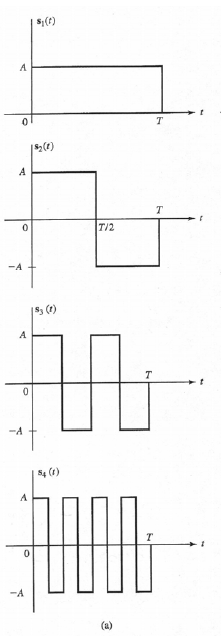
\includegraphics[scale = 1]{4 sequenze ortogonali.PNG}
\end{figure}

costituite, cioè, da una successione di segmenti, 
in cui il segnale vale +1 o -1 (+A e -A in figura). \newline 

Segnali di questo tipo, possono essere convenzionalmente, denominati sequenze ortogonali. \newline 

Per generare un insieme di M sequenze ortogonali, possono essere utilizzate le matrici di Hadamard. \newline 

\begin{tcolorbox}
    In questa sezione utilizziamo la notazione del prof per indicare le matrici. \newline 

    Quindi indicheremo le matrici con il grassetto.
\end{tcolorbox}

La matrice di Hadamard di ordine 2 ha la seguente struttura: 

{
    \Large 
    \begin{equation}
        \textbf{H}_2 
        = 
        \begin{bmatrix}
            1 & 1 \\
            1 & -1
        \end{bmatrix}
    \end{equation}
}

\begin{tcolorbox}
    Leggendo le colonne di $\textbf{H}_2 $ i conti portano perchè le prima colonna ha valori 
    $\begin{bmatrix}
        1 \\
        1
    \end{bmatrix}$
    che equivalgono i valori della prima sequenza nella figura $s_1 (t)$, cioè: 
    $\begin{bmatrix}
        A \\
        A
    \end{bmatrix}
    $, invece per la seconda colonna di $\textbf{H}_2 $ ha valori 
    $\begin{bmatrix}
        1 \\
        -1
    \end{bmatrix}
    $, nella figura $s_2 (t)$ ha valori 
    $\begin{bmatrix}
        A \\
        -A
    \end{bmatrix}
    $
\end{tcolorbox}

A partire da essa, supposto che n sia una potenza di 2, si utilizza la seguente procedura iterativa: 

{
    \Large 
    \begin{equation}
        \textbf{H}_{2n}
        = 
        \begin{bmatrix}
            \textbf{H}_{n} & \textbf{H}_{n} \\
            \textbf{H}_{n} & - \textbf{H}_{n}
        \end{bmatrix}
    \end{equation}
}

Così, ad esempio, la matrice di Hadamard di ordine 4 si ottiene come: 

{
    \Large 
    \begin{equation}
          \textbf{H}_{4}
        = 
        \begin{bmatrix}
            \textbf{H}_{2} & \textbf{H}_{2} \\
            \textbf{H}_{2} & - \textbf{H}_{2}
        \end{bmatrix}
        =
        \begin{bmatrix}
            1 & 1 & 1 & 1 \\
            1 & -1 & 1 & -1 \\
            1 & 1 & -1 & -1 \\
            1 & -1 & -1 & 1 
        \end{bmatrix}
    \end{equation}
}


In questa maniera, per ogni colonna e dividendo ogni cella per un multiplo di T, otteniamo delle sequenze ortogonali tra loro. \newline 

A partire dalla matrice che identifica l'insieme ortogonale, 
è immediato ottenere la matrice che identifica l'insieme bi-ortogonale. \newline 

Indicato con $\textbf{H}_{\frac{M}{2}}$, 
una matrice di Hadamard di ordine $\frac{M}{2}$ si avrà infatti la matrice dell'insieme bi-ortogonale: 

{
    \Large 
    \begin{equation}
        \left. \textbf{H}_{2} \right|_{biortogonale}
        = 
        \begin{bmatrix}
            \textbf{H}_{\frac{M}{2}} \\
            - \textbf{H}_{\frac{M}{2}}
        \end{bmatrix}
    \end{equation}
}

Considerando M = 4, 
la matrice di Hadamard di ordine $\frac{M}{2}$ sarà: 

{
    \Large 
    \begin{equation}
          \left. \textbf{H}_{4} \right|_{biortogonale}
        = 
        \begin{bmatrix}
            1 & 1  \\
            1 & -1 \\
            1 & 1  \\
            1 & -1 
        \end{bmatrix}
    \end{equation}
}


Per ottenere M forme d'onda trans-ortogonali, 
si ottiene eliminando la prima colonna della matrice ortogonale da cui deriva. \newline 

Quindi, per M = 4, da: 

{
    \Large 
    \begin{equation}
          \textbf{H}_{4}
        = 
        \begin{bmatrix}
            \textbf{H}_{2} & \textbf{H}_{2} \\
            \textbf{H}_{2} & - \textbf{H}_{2}
        \end{bmatrix}
        =
        \begin{bmatrix}
            1 & 1 & 1 & 1 \\
            1 & -1 & 1 & -1 \\
            1 & 1 & -1 & -1 \\
            1 & -1 & -1 & 1 
        \end{bmatrix}
    \end{equation}
}

diventa: 

{
    \Large 
    \begin{equation}
          \textbf{H}_{4}
        =
        \begin{bmatrix}
            1 & 1 & 1 \\
            -1 & 1 & -1 \\
            1 & -1 & -1 \\
            -1 & -1 & 1 
        \end{bmatrix}
    \end{equation}
}

\newpage 

\section{Alcune considerazioni sullo spettro e la banda occupata}
\footnote{Slide del prof | Formati di trasmissione numerica | pag 30 - 32\\  
Appunti di Damiano | pag 30 - 32\\
Slide | Formati di trasmissione numerica | pag  30 - 32\\
Appunti | 2025-04-01 | pag 4
}

In questo paragrafo ci limitiamo a riportare, senza dimostrazione, l'effetto sull'occupazione spettrale (banda) di un incremento del valore di M (cardinalità del formato di trasmissione). \newline 

Nelle trasmissione M-arie, 
ogni simbolo sostituisce k: 

{
    \Large 
    \begin{equation}
        k = \log_{2} (M)
    \end{equation}
}

dove k sono i bit per ogni simbolo. \newline

La durata di ciascun simbolo M-aria è k volte maggiore della durata del singolo bit. \newline 

Nella trasmissione binaria, si possono avere variazione ogni $T_b$ secondi, 
mentre nella trasmissione M-aria, il segnale può variare ogni T: 

{
    \Large 
    \begin{equation}
        T = T_b \cdot \log_{2} (M)
    \end{equation}
}

dove con T è in secondi. \newline 

k è minore di T, quindi, nella trasmissione M-aria ci vorrà più tempo per inviare un simbolo. \newline 

Il simbolo M-aria ha un'occupazione spettrale significativa $\log_{2} (M)$ volte più piccola della corrispondente occupazione spettrale del segnale binario. \newline 

A titolo di esempio si riporta l'andamento dello spettro di potenza per il formato 2-ASK avendo posto $R = \frac{1}{T_b}$: 

\begin{figure}[h]
    \centering
    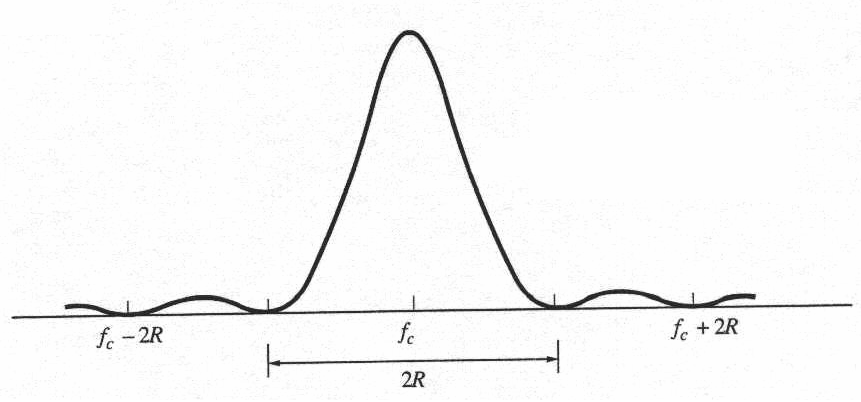
\includegraphics[scale = 1]{Settro di potenza 2-ASK.png}
\end{figure}

Se si considera un valore di M maggiore di 2, la forma dello spettro rimane inalterata, ma si riduce la banda intorno alla frequenza $f_c$. \newline 

Ma, l'aumenta M significa anche ridurre la qualità della trasmissione. \newline 

Generalmente questo principio vale nella maggior parte dei formati, 
tranne i formati ortogonali o derivati dagli ortogonali. \newline 

Ad esempio nella PPM, all'aumentare di M si allarga la banda. \newline 

Inoltre, all'aumentare dalla banda, la qualità migliora e si abbassa la probabilità di errore. \newline 

\begin{tcolorbox}
    Il vincolo della banda è un problema nelle trasmissione senza fili, 
    ma nella fibra ottica abbiamo banda "illimitata", quindi non è un problema e possiamo implementare una PPM con M molto elevato.
\end{tcolorbox}

\newpage 
